
\documentclass[10pt]{article}
\usepackage[a4paper,landscape,top=1.6cm,bottom=1.6cm,left=1.8cm,right=1.8cm]{geometry}
\usepackage[utf8]{inputenc}
\usepackage[T1]{fontenc}
\usepackage{lmodern}
\usepackage{microtype}
\usepackage{amsmath,amssymb}
\usepackage{xcolor}
\usepackage[most,breakable]{tcolorbox}
\usepackage{multicol}
\usepackage{booktabs,tabularx,longtable,array,colortbl}
\usepackage{fancyhdr}
\usepackage{enumitem}
\usepackage{lastpage}
\usepackage[hidelinks]{hyperref}
\usepackage{tikz}
\usetikzlibrary{arrows.meta,positioning,calc}
\definecolor{TealBg}{HTML}{E0F2F1}
\definecolor{NavyBg}{HTML}{E8EEFF}

%% ── Colours ─────────────────────────────────────────────────────────────────
\definecolor{Navy}{HTML}{0D2B6B}
\definecolor{Sky}{HTML}{1976D2}
\definecolor{Teal}{HTML}{00695C}
\definecolor{FGreen}{HTML}{2E7D32}
\definecolor{Amber}{HTML}{E65100}
\definecolor{DRed}{HTML}{B71C1C}
\definecolor{Purple}{HTML}{6A1B9A}
\definecolor{Indigo}{HTML}{303F9F}
\definecolor{LBg}{HTML}{F5F7FA}
\definecolor{BBg}{HTML}{E3F2FD}
\definecolor{GBg}{HTML}{E8F5E9}
\definecolor{RBg}{HTML}{FFEBEE}
\definecolor{ABg}{HTML}{FFF8E1}
\definecolor{IBg}{HTML}{E8EAF6}
\definecolor{TabOdd}{HTML}{EEF2F7}
\definecolor{TGcol}{HTML}{E65100}
\definecolor{QGcol}{HTML}{1565C0}
\definecolor{FGcol}{HTML}{2E7D32}

%% ── tcolorbox styles ────────────────────────────────────────────────────────
\tcbuselibrary{skins,breakable}
\tcbset{
  mybox/.style 2 args={
    enhanced, arc=3pt, boxrule=0.7pt,
    fonttitle=\bfseries\small\color{white},
    colbacktitle=#1, colframe=#1, colback=#2,
    lefttitle=5pt, toptitle=3pt, bottomtitle=3pt,
    top=5pt, bottom=5pt, left=6pt, right=6pt,
    before skip=5pt, after skip=5pt, breakable
  }
}
\newcommand{\navybox}[2]{\begin{tcolorbox}[mybox={Navy}{LBg},title={#1}]#2\end{tcolorbox}}
\newcommand{\skybox}[2]{\begin{tcolorbox}[mybox={Sky}{BBg},title={#1}]#2\end{tcolorbox}}
\newcommand{\tealbox}[2]{\begin{tcolorbox}[mybox={Teal}{LBg},title={#1}]#2\end{tcolorbox}}
\newcommand{\greenbox}[2]{\begin{tcolorbox}[mybox={FGreen}{GBg},title={#1}]#2\end{tcolorbox}}
\newcommand{\amberbox}[2]{\begin{tcolorbox}[mybox={Amber}{ABg},title={#1}]#2\end{tcolorbox}}
\newcommand{\redbox}[2]{\begin{tcolorbox}[mybox={DRed}{RBg},title={#1}]#2\end{tcolorbox}}
\newcommand{\purplebox}[2]{\begin{tcolorbox}[mybox={Purple}{LBg},title={#1}]#2\end{tcolorbox}}
\newcommand{\indigobox}[2]{\begin{tcolorbox}[mybox={Indigo}{IBg},title={#1}]#2\end{tcolorbox}}

%% ── Page header helper ───────────────────────────────────────────────────────
\newcommand{\pagehead}[2]{%
  \begin{tcolorbox}[enhanced,arc=0pt,outer arc=0pt,boxrule=0pt,
    colback=Navy,colframe=Navy,
    top=5pt,bottom=5pt,left=8pt,right=8pt,
    before skip=0pt,after skip=10pt]
  {\color{white}\large\bfseries #1}%
  \ifx\relax#2\relax\else\\[1pt]{\color{blue!30!white}\small #2}\fi
  \hfill{\color{blue!20!white}\footnotesize Synthetic Financial Time Series $\cdot$ UPC}
  \end{tcolorbox}}

%% ── Footer ───────────────────────────────────────────────────────────────────
\pagestyle{fancy}\fancyhf{}\renewcommand{\headrulewidth}{0pt}
\fancyfoot[C]{\small\color{gray!70}
  Page~\thepage\ of~\pageref{LastPage}\quad$\cdot$\quad
  Synthetic Financial Time Series --- GAN Benchmark\quad$\cdot$\quad UPC Research}

%% ── Citations ───────────────────────────────────────────────────────────────
%% \tcite{N} → superscript [N] that hyperlinks to bibliography entry R:N
\newcommand{\tcite}[1]{%
  \hyperlink{R:#1}{\textsuperscript{\scriptsize\textbf{[#1]}}}}
%% packages for reference list
\usepackage{enumitem}
\usepackage{multicol}

%% ── Misc ─────────────────────────────────────────────────────────────────────
\setlength{\parindent}{0pt}\setlength{\parskip}{4pt}\setlength{\columnsep}{14pt}
\setlist[itemize]{noitemsep,topsep=2pt,leftmargin=14pt,label=\textbullet}
\setlist[enumerate]{noitemsep,topsep=2pt,leftmargin=16pt}
\newcommand{\E}{\mathbb{E}}
\newcommand{\R}{\mathbb{R}}
\newcommand{\norm}[1]{\left\|#1\right\|}

%% ═══════════════════════════════════════════════════════════════════════════════
\begin{document}

%% ─── Page 1: Title ───────────────────────────────────────────────────────────
\thispagestyle{empty}
\pagecolor{Navy}\color{white}
\vspace*{2.0cm}
\begin{center}
{\fontsize{26}{32}\selectfont\bfseries Synthetic Financial Time Series Generation\par}
\vspace{0.4cm}
{\Large GAN Benchmark:\quad TimeGAN\ \ $\cdot$\ \ QuantGAN\ \ $\cdot$\ \ FinGAN\par}
\vspace{0.2cm}
{\large BRICS Emerging Market Indices\par}
\vspace{0.7cm}
\textcolor{blue!40!white}{\rule{0.65\textwidth}{0.5pt}}
\vspace{0.7cm}

\begin{tabular}{r@{\hspace{10pt}}l}
  \textbf{Collaboration}  & Universitat Polit\`{e}cnica de Catalunya (UPC) \\[4pt]
  \textbf{Document type}  & Project Status \& In-Depth Technical Review \\[4pt]
  \textbf{Purpose}        & Paper publication preparation \\[4pt]
  \textbf{Models}         & TimeGAN (RNN) $\cdot$ QuantGAN (TCN-WGAN-GP) $\cdot$ FinGAN (CNN-WGAN-GP) \\[4pt]
  \textbf{Markets}        & BOVESPA $\cdot$ FTSE JSE $\cdot$ MSCI $\cdot$ NIFTY50 $\cdot$ SHANGHAI \\[4pt]
  \textbf{Generated}      & 2026-08-30 \\
\end{tabular}
\end{center}
\clearpage\pagecolor{white}\color{black}

%% ─── Page 2: Project Overview ────────────────────────────────────────────────
\pagehead{Project Status Overview}
         {Research context $\cdot$ data pipeline $\cdot$ model status $\cdot$ open tasks}

\begin{multicols}{2}

\navybox{Research Goal}{%
\begin{itemize}
  \item Benchmark three GAN architectures for synthetic financial log-return generation
  \item Evaluate on 5 BRICS emerging-market indices (multi-market generalisation)
  \item Use literature-anchored hyperparameter floors (Gulrajani 2017); validate temporal robustness with walk-forward evaluation (CTBench protocol)
  \item Compare stylized-fact reproduction: fat tails, volatility clustering, long memory
  \item Prepare peer-reviewed paper in collaboration with UPC
\end{itemize}}

\skybox{Data Pipeline}{%
\begin{itemize}
  \item Source: 5 CSV files --- BOVESPA, FTSE JSE, MSCI, NIFTY50, SHANGHAI
  \item Feature: daily log return $r_t = \ln(P_t / P_{t-1})$
  \item \textbf{No outlier clipping} applied to log returns (deliberate --- see Code Audit)
  \item Temporal 80\,/\,10\,/\,10 split (no shuffle) --- saved as Parquet files; train set used for GAN training
  \item GAN training: 15 models (3 GANs $\times$ 5 markets); each model trains on 128-step windows from its own market only --- no cross-market data mixing
  \item Walk-forward evaluation: 5 rolling folds per market on that market's test series (CTBench protocol); model retrained each fold
\end{itemize}}

\columnbreak

\begin{tcolorbox}[mybox={TGcol}{ABg},title={TimeGAN}]
Yoon et al.\ (2019)\tcite{4}, NeurIPS 32. 4-phase training (autoencoder $\to$ supervisor $\to$ joint GAN) using GRU networks. BCE loss + moment matching. MinMax $[0,1]$ normalisation.
\textcolor{DRed}{\bfseries\small Current: epochs=5 (far too low --- see Audit)}
\end{tcolorbox}

\begin{tcolorbox}[mybox={QGcol}{BBg},title={QuantGAN}]
Wiese et al.\ (2020)\tcite{5}, Quantitative Finance. WGAN-GP + TCN with causal dilated convolutions. Adam $\beta_1=0$, $\beta_2=0.9$, \textbf{n\_critic=5} (Gulrajani\tcite{3} 2017 floor), $\lambda_\text{gp}=10$.
\end{tcolorbox}

\begin{tcolorbox}[mybox={FGcol}{GBg},title={FinGAN}]
Custom CNN-WGAN-GP. Generator: FC $\to$ 3$\times$ \texttt{ConvTranspose1d}. Critic: \texttt{Conv1d} + LayerNorm. seq\_len must be divisible by 8. Same Adam/WGAN-GP settings as QuantGAN.
\end{tcolorbox}

\greenbox{Pipeline Status}{%
\begin{itemize}
  \item \textbf{DONE:} Reproducibility seeds; deprecated API fixes; literature-anchored hyperparameter floors (n\_critic=5, $\lambda_\text{gp}=10$)
  \item \textbf{DONE:} \texttt{FinancialMetrics} rewritten with time-series-aware tests
  \item \textbf{DONE:} \texttt{n\_critic} fixed at 5 for QuantGAN and FinGAN (Gulrajani\tcite{3} 2017 floor)
  \item \textbf{DONE:} Walk-forward validation (\texttt{walk\_forward\_evaluate()}, CTBench protocol, 5 rolling folds)
  \item \textbf{TODO:} Re-run pipeline to regenerate results with updated metric schema
  \item \textbf{TODO:} Increase TimeGAN epochs ($\geq 50$--$100$ per phase)
\end{itemize}}

\end{multicols}

\clearpage

%% ─── Page 3: Financial Time Series from Scratch ──────────────────────────────
\pagehead{The Problem --- Financial Time Series from First Principles}
         {Understanding the data before understanding the models}

\begin{multicols}{2}

\navybox{What is a Financial Time Series?}{%
A financial time series is simply a sequence of numbers measured over time.
For a stock or index: $P_1, P_2, \ldots, P_T$ where $P_t$ is the closing price on day $t$.

\smallskip
\textbf{Problem with raw prices:} they grow over time (non-stationary), making comparisons across periods misleading. Statistical models require (approximate) stationarity.}

\skybox{Why Log Returns?}{%
Instead of prices we compute the \textbf{log return} for each day:
\begin{equation*}
  r_t = \ln\!\left(\frac{P_t}{P_{t-1}}\right) = \ln P_t - \ln P_{t-1}
\end{equation*}

\textbf{Why the logarithm?}
\begin{enumerate}
  \item \textit{Additivity:}\ $r_{1\to3} = r_{1\to2} + r_{2\to3}$ exactly (simple returns do not add).
  \item \textit{Approximation:}\ $\ln(P_t/P_{t-1}) \approx (P_t-P_{t-1})/P_{t-1}$ for small moves.
  \item \textit{Stationarity:}\ Log returns fluctuate around zero with no long-run trend.
\end{enumerate}}

\redbox{The Core Problem: Returns Are NOT Normal}{%
The simplest model: $r_t \overset{\text{i.i.d.}}{\sim} \mathcal{N}(\mu,\sigma^2)$.
This is the foundation of Black--Scholes and many classical models.
\textbf{It is empirically wrong in the tails.}

Under $\mathcal{N}(0,\sigma^2)$ with $\sigma \approx 1.2\%$:
\begin{itemize}
  \item A day with $|r| > 3\sigma \approx 3.6\%$ should occur $\approx 0.27\%$ of days \\ $\Rightarrow$ roughly 1 day per year.
  \item Reality: 3--5$\times$ more frequent (\textbf{heavy tails}).
  \item A ``$5\sigma$ crash'': under Gaussian $\approx$ once every \textbf{14\,000 years}; \\ in practice: several times per decade.
\end{itemize}
The 2008 crisis was described as a ``25-sigma event'' by some risk systems --- probabilistically impossible under Gaussian assumptions.}

\columnbreak

\tealbox{What Are Stylized Facts?}{%
Cont (2001)\tcite{7} coined the term \textbf{stylized facts}: statistical properties that appear consistently across virtually all financial markets and time periods. They are the fingerprint of financial returns.

\textbf{Any generative model claiming to produce realistic synthetic returns MUST reproduce them.}

The five most important:
\begin{enumerate}
  \item \textbf{Heavy tails:}\ $P(|r|>x) \sim x^{-\alpha}$ (Pareto tail, $\alpha \approx 3$--$5$) $\Rightarrow$ kurtosis $\gg 3$.
  \item \textbf{Near-zero autocorrelation:}\ $\text{Corr}(r_t, r_{t+k}) \approx 0$ for $k \geq 1$ (efficient market).
  \item \textbf{Volatility clustering:}\ $\text{Corr}(|r_t|, |r_{t+k}|) > 0$ for $k = 1,\ldots,100+$. Large moves beget large moves.
  \item \textbf{Long memory:}\ ACF of $|r_t|$ decays as $k^{-\beta}$, $\beta \in (0,1)$; Hurst exponent $H > 0.5$.
  \item \textbf{Negative skewness:}\ crashes are sharper than rallies ($\text{skew}(r) < 0$ for equity indices).
\end{enumerate}}

\purplebox{Why Generate Synthetic Data?}{%
If real data exists, why generate synthetic data?
\begin{itemize}
  \item \textbf{Data augmentation:}\ deep learning models need large datasets; markets produce $\sim$250 observations/year.
  \item \textbf{Stress testing:}\ banks test risk models under extreme scenarios not in historical data.
  \item \textbf{Privacy:}\ real data may be proprietary; synthetic data with the same statistical properties can be shared freely.
  \item \textbf{Scenario generation:}\ sample many plausible futures for portfolio optimisation.
\end{itemize}
\textbf{The challenge:} a Gaussian generator fails immediately (wrong tails, no clustering). This motivates deep generative models.}

\end{multicols}

\clearpage

%% ─── Page 4: What is a GAN? ──────────────────────────────────────────────────
\pagehead{The Solution Candidate: What is a Generative Adversarial Network?}
         {From the counterfeiter--detective analogy to the minimax formulation (Goodfellow et al., 2014)}

\begin{multicols}{2}

\navybox{The Core Idea --- A Two-Player Game}{%
Goodfellow et al.\ (2014)\tcite{1} proposed training \textbf{two} neural networks that compete:

\smallskip
\textbf{Generator} $G$: takes random noise $z \sim p_z$ $\to$ outputs fake sample $G(z) = \tilde{x}$.
\textbf{Discriminator} $D$: given a sample (real or fake) $\to$ outputs $D(x) \in [0,1]$ (probability of being real).

\smallskip
\textbf{Analogy:} Counterfeiter ($G$) makes fake banknotes; detective ($D$) tries to spot them.
Both improve iteratively until fakes are indistinguishable.

\smallskip
The \textbf{minimax objective}:
\begin{equation*}
  \min_G\ \max_D\ V(D,G) =
  \underbrace{\E_{x \sim p_\text{data}}\!\bigl[\log D(x)\bigr]}_{\text{reward } D \text{ for real}}
  +
  \underbrace{\E_{z \sim p_z}\!\bigl[\log(1 - D(G(z)))\bigr]}_{\text{penalise } G \text{ when caught}}
\end{equation*}

Reading each term:
\begin{itemize}
  \item $D$ \emph{maximises}: wants $D(x_\text{real}) \to 1$ and $D(G(z)) \to 0$.
  \item $G$ \emph{minimises}: wants $D(G(z)) \to 1$ (fool $D$).
\end{itemize}

At the \textbf{Nash equilibrium} (Goodfellow et al., 2014, Proposition 1):
\begin{equation*}
  D^*(x) = \frac{p_\text{data}(x)}{p_\text{data}(x)+p_g(x)} = \tfrac{1}{2}\ \forall\,x
  \quad\Longrightarrow\quad p_g = p_\text{data}
\end{equation*}
The generator has perfectly learnt the real distribution.}

\redbox{Critical Problem: Vanishing Gradients \& Mode Collapse}{%
\textbf{Mode collapse:}\ $G$ learns to output only a few samples that reliably fool $D$, ignoring the true diversity of $p_\text{data}$.

\textbf{Vanishing gradients:}\ The GAN loss uses Jensen--Shannon (JS) divergence internally:
\begin{equation*}
  \text{JS}(p_\text{data} \| p_g) = \log 2 \quad\text{when } \text{supp}(p_\text{data}) \cap \text{supp}(p_g) = \varnothing
\end{equation*}
A \textit{constant} has zero derivative with respect to $G$'s parameters $\Rightarrow$ $G$ receives no learning signal.

\textbf{In practice:} early in training, if $G$ produces very different-looking samples from reality, $D$ immediately says ``fake'' with no useful feedback on \emph{how} $G$ should improve.}

\columnbreak

\skybox{What Makes GANs Suitable for Financial Returns?}{%
Unlike parametric models (GARCH, EVT), a GAN:
\begin{itemize}
  \item Makes \textbf{no distributional assumption} about the shape of returns; learns $p_\text{data}$ implicitly.
  \item Can model arbitrarily complex joint distributions $p(r_1, r_2, \ldots, r_T)$, capturing both the marginal distribution \emph{and} temporal dependencies.
  \item Scales to multivariate settings without specifying a copula.
\end{itemize}

\textbf{The GAN sees sequences, not points.}
A window $[r_1, r_2, \ldots, r_{128}]$ is the training unit. $D$ learns to recognise temporal patterns: bursts of high volatility, calm periods. $G$ must generate sequences exhibiting those patterns.

This is what distinguishes GAN-based generators from models that generate each timestep independently (which would produce no volatility clustering even if the marginal distribution were correct).}

\navybox{Three Architectural Choices in This Benchmark}{%
\begin{center}
\renewcommand{\arraystretch}{1.4}
\begin{tabular}{@{}lll@{}}
\toprule
\textbf{Model} & \textbf{Backbone} & \textbf{Key mechanism} \\
\midrule
\textcolor{TGcol}{\textbf{TimeGAN}}  & GRU (recurrent)  & Latent embedding space \\
\textcolor{QGcol}{\textbf{QuantGAN}} & TCN (causal dil.) & Long receptive field via dilation \\
\textcolor{FGcol}{\textbf{FinGAN}}   & CNN deconvolution & Noise $\to$ sequence via upsampling \\
\bottomrule
\end{tabular}
\end{center}}

\end{multicols}

\clearpage

%% ─── Page 5: WGAN-GP ─────────────────────────────────────────────────────────
\pagehead{Better Training: The Wasserstein GAN and Gradient Penalty}
         {Arjovsky et al.\ (2017)\tcite{2} ICML $\cdot$ Gulrajani et al.\ (2017)\tcite{3} NeurIPS}

\begin{multicols}{2}

\navybox{A Better Distance Between Distributions}{%
The JS divergence fails because it equals $\log 2$ (a constant) when supports do not overlap --- giving $G$ zero gradient.

\textbf{Wasserstein-1 distance} (``Earth Mover's distance''):
\begin{equation*}
  W(p, q) = \inf_{\gamma \in \Pi(p,q)} \E_{(x,y)\sim\gamma}\bigl[\norm{x - y}\bigr]
\end{equation*}
where $\Pi(p,q)$ is the set of all joint distributions with marginals $p$ and $q$.

\textbf{Physical intuition:}
Think of $p_\text{data}$ and $p_g$ as two piles of sand.
$W$ is the minimum total work (mass $\times$ distance) needed to reshape one pile into the other.

\textbf{Why is this better?}
\begin{itemize}
  \item $W$ is continuous and \emph{always} provides a gradient signal, even when distributions do not overlap.
  \item $W$ correlates with visual generation quality, unlike the JS loss which can plateau.
\end{itemize}}

\skybox{Kantorovich--Rubinstein Duality --- Making $W$ Tractable}{%
The infimum over all joint distributions in $W(p,q)$ is computationally intractable.
The key theorem (Kantorovich--Rubinstein):
\begin{equation*}
  W(p_\text{data}, p_g)
  = \sup_{\norm{f}_L \leq 1}
    \Bigl(\E_{x \sim p_\text{data}}[f(x)] - \E_{x \sim p_g}[f(x)]\Bigr)
\end{equation*}
where the supremum is over all \textbf{1-Lipschitz} functions:
\begin{equation*}
  \norm{f}_L \leq 1 \;\Longleftrightarrow\; |f(x) - f(y)| \leq \norm{x - y}\quad\forall\,x,y
\end{equation*}
\textbf{Implication:} the WGAN \textbf{Critic} $D$ (now unbounded, not a probability) plays the role of $f$.
We parameterise $D$ with a neural network and train it to approximate the optimal $f$.

WGAN training objective:
\begin{equation*}
  \min_G\ \max_{\norm{D}_L \leq 1}\ \E_{x \sim p_\text{data}}[D(x)] - \E_{z \sim p_z}[D(G(z))]
\end{equation*}}

\columnbreak

\tealbox{Gradient Penalty (Gulrajani et al., 2017)}{%
The original WGAN enforces the Lipschitz constraint by weight clipping (crude, slow).
WGAN-GP uses a differentiable penalty instead:
\begin{equation*}
  \mathcal{L}_\text{GP}
  = \lambda \cdot \E_{\hat{x} \sim p_{\hat{x}}}\!\left[
      \Bigl(\norm{\nabla_{\hat{x}}\, D(\hat{x})}_2 - 1\Bigr)^2\right]
\end{equation*}
where the interpolated point and mixing coefficient are:
\begin{equation*}
  \hat{x} = \varepsilon\, x_\text{real} + (1-\varepsilon)\, x_\text{fake},
  \qquad \varepsilon \sim \mathcal{U}[0,1],\quad \lambda = 10
\end{equation*}
The penalty pushes $\norm{\nabla D(\hat{x})}_2 \to 1$ throughout training.

\textbf{Full training losses:}
\begin{align*}
  \mathcal{L}_D &= \E[D(\tilde{x})] - \E[D(x)] + \lambda\,\mathcal{L}_\text{GP}
                   \quad\text{($D$ minimises $-\mathcal{L}_D$)} \\
  \mathcal{L}_G &= -\E[D(G(z))]
\end{align*}
\textbf{n\_critic\,$=3$:}\ $D$ is updated 3$\times$ per $G$ update. This ensures $D$ tracks the true Wasserstein distance accurately before $G$ uses the gradient signal.}

\navybox{Adam Optimiser: Why $\beta_1 = 0$?}{%
Standard Adam uses $\beta_1 = 0.9$ (momentum) and $\beta_2 = 0.999$ (RMS scaling). Gulrajani et al.\ (2017)\tcite{3} recommend $\beta_1 = 0$, $\beta_2 = 0.9$.

In adversarial training, gradients \emph{reverse direction frequently}: in one step $D$ pushes $G$ one way, in the next step their roles shift. Momentum ($\beta_1 > 0$) accumulates past gradients and pushes in the \emph{wrong} direction, causing oscillations. Setting $\beta_1 = 0$ disables momentum; only the current gradient scaled by $\beta_2$-RMS is used.}

\amberbox{Why No BatchNorm in the WGAN-GP Critic?}{%
BatchNorm normalises across the batch: $\hat{x}_i = (x_i - \mu_\text{batch})/\sigma_\text{batch}$.
When computing $\mathcal{L}_\text{GP}$, the gradient $\nabla_{\hat{x}} D(\hat{x})$ must reflect how $D$ responds to a \emph{single} interpolated point. BatchNorm introduces a dependency on \emph{other samples} in the batch, corrupting the gradient norm calculation and breaking the Lipschitz enforcement.

Solution: use \textbf{LayerNorm} (normalises per sample across features), which has no batch dependency. Both QuantGAN and FinGAN use LayerNorm in the critic.}

\end{multicols}

\clearpage

%% ─── Page 6: TimeGAN ────────────────────────────────────────────────────────
\pagehead{TimeGAN: Making the GAN Time-Aware}
         {Yoon, Jarrett \& van der Schaar (2019) NeurIPS 32 --- GRU + embedding space + 4-phase training}

\begin{multicols}{2}

\navybox{Why a Plain GAN Fails on Time Series}{%
A basic GAN generates each window independently from a noise vector. It \emph{can} match the marginal distribution $p(r_t)$ (correct tails, correct scale), but has no mechanism to enforce that consecutive steps within a window exhibit temporal patterns like volatility clustering.

\textbf{Analogy:}\ Writing a novel by choosing each word independently from a realistic vocabulary. Individual words are real English, but the sequence is incoherent.}

\skybox{What is a GRU? (From Scratch)}{%
A \textbf{GRU} (Gated Recurrent Unit) processes a sequence step by step, maintaining a ``hidden state'' $h_t$ --- a running summary of all past inputs.

At each step $t$, given $x_t$ (current input) and $h_{t-1}$ (previous summary):
\begin{align*}
  r_t &= \sigma\!\bigl(W_r [h_{t-1},\, x_t]\bigr) && \text{reset gate} \\
  z_t &= \sigma\!\bigl(W_z [h_{t-1},\, x_t]\bigr) && \text{update gate} \\
  \tilde{h}_t &= \tanh\!\bigl(W [r_t \odot h_{t-1},\, x_t]\bigr) && \text{candidate state} \\
  h_t &= (1-z_t)\odot h_{t-1} + z_t \odot \tilde{h}_t && \text{new hidden state}
\end{align*}
The update gate $z_t$ controls how much past information to keep vs.\ replace. The key property: $h_t$ is a \emph{compressed summary} of all inputs so far.}

\navybox{Key Innovation: Generating in Embedding Space}{%
TimeGAN trains the GAN in a \textbf{learned latent space} $\mathcal{H}$, not in the raw return space $\mathcal{X}$.

\textbf{Why?}\ Raw returns are noisy. A smooth latent space is easier to model with a GAN. Moreover, a \emph{Supervisor} network is trained to predict $h_{t+1}$ from $h_t$, embedding the temporal dynamics into $\mathcal{H}$. $G$ then generates sequences in $\mathcal{H}$ that follow these learned dynamics.}

\columnbreak

\tealbox{The Four-Phase Training Algorithm}{%
\textbf{Phase 1 --- Autoencoder} (epochs\,//\,2 steps):
\begin{itemize}
  \item Embedder $e: \mathcal{X} \to \mathcal{H}$; Recovery $\hat{r}: \mathcal{H} \to \tilde{\mathcal{X}}$
  \item $\mathcal{L}_R = \norm{X - \hat{r}(e(X))}^2$ \quad (reconstruction)
\end{itemize}

\textbf{Phase 2 --- Supervisor} (epochs\,//\,2 steps):
\begin{itemize}
  \item Supervisor $s: \mathcal{H} \to \hat{\mathcal{H}}$\ (step-ahead prediction in latent space)
  \item $\mathcal{L}_S = \norm{H_{t+1} - s(H_t)}^2$
\end{itemize}

\textbf{Phase 3 --- Joint Adversarial Training} (epochs steps):
\begin{equation*}
  z \to G(z)=\hat{H} \to s(\hat{H}) \to \hat{r}(\cdot) \to \tilde{X}
\end{equation*}
\begin{align*}
  \mathcal{L}_G &= \mathcal{L}_U + 100\sqrt{\mathcal{L}_S} + 100\,\mathcal{L}_V \\[2pt]
  \mathcal{L}_U &= -\E\!\bigl[\log D(s(G(z)))\bigr] \quad\text{(adversarial)} \\
  \mathcal{L}_V &= |\mu_H - \mu_{\hat{H}}| + |\sigma_H - \sigma_{\hat{H}}| \quad\text{(moments)}
\end{align*}
Discriminator: $\mathcal{L}_D = \text{BCE}\!\bigl(D(H_\text{real}),1\bigr) + \text{BCE}\!\bigl(D(H_\text{fake}),0\bigr)$}

\redbox{Critical Issue: Training Budget}{%
With the current setting \texttt{epochs = 5}:
\begin{itemize}
  \item Phase 1 gets $5 // 2 = 2$ gradient steps.
  \item Phase 2 gets $5 // 2 = 2$ gradient steps.
\end{itemize}
\textbf{A GRU cannot converge in 2 steps.}\ The embedding space $\mathcal{H}$ is essentially random noise $\Rightarrow$ Phase 3 trains a GAN on top of garbage.

Yoon et al.\ (2019)\tcite{4} use \textbf{5\,000--10\,000 iterations per phase}. TimeGAN's poor ranking (avg\_rank\,$= 2.36$) almost certainly reflects this budget, not its architecture.

\textbf{Fix required:}\ epochs\,$\geq 50$ (or add explicit per-phase iteration counts).}

\end{multicols}

\clearpage

%% ─── Page 7: QuantGAN & FinGAN ───────────────────────────────────────────────
\pagehead{QuantGAN \& FinGAN: Convolutional Approaches to Time Series Generation}
         {Building from convolutions to causal dilated TCNs to CNN-WGAN-GP generators}

\begin{multicols}{2}

\navybox{What is a Convolution? (From Scratch)}{%
A 1D convolution slides a small filter (kernel) of size $K$ over a sequence:
\begin{equation*}
  \text{out}[t] = \sum_{k=0}^{K-1} w_k \cdot \text{in}[t - k]
\end{equation*}
Think of it as a magnifying glass that scans the time series, highlighting patterns of a specific shape. The weights $w_0,\ldots,w_{K-1}$ are learnt from data.

\textbf{Causal constraint} (no future leakage):\ only inputs at $t, t-1, \ldots, t-(K-1)$ are used.

\textbf{Dilated convolution} (skip steps to see further back cheaply):
\begin{equation*}
  \text{out}[t] = \sum_{k=0}^{K-1} w_k \cdot \text{in}[t - k \cdot d]
\end{equation*}
With dilation $d=1,2,4,8,\ldots$ and $K=2$: receptive field grows as $1+\sum_l 2^l$, doubling per layer with no extra parameters.}

\begin{tcolorbox}[mybox={QGcol}{BBg},title={QuantGAN --- TCN-based WGAN-GP (Wiese et al., 2020)}]
\textbf{Key innovation:}\ replace GRU with a Temporal Convolutional Network (TCN) --- fully parallelisable, no vanishing-gradient-across-time problem.

\textbf{Generator:} $z$ (\texttt{noise\_dim=100}) $\to$ \texttt{Linear} $\to$ reshape $(C, T/4)$ $\to$ \texttt{ConvTranspose1d}$\times$2 (stride 2, $2\times$ upsample) $\to$ TCN (3 residual blocks, dilations 1/2/4) $\to$ \texttt{Conv1d(1)} $\to$ \texttt{Tanh} $\to \tilde{x}$

\textbf{Critic:} $x$ $(T\times 1)$ $\to$ permute $\to$ TCN (3 blocks) $\to$ \texttt{AdaptiveAvgPool1d(1)} $\to$ \texttt{Linear(128)} $\to$ \texttt{LeakyReLU} $\to$ \texttt{Linear(1)}

\texttt{AdaptiveAvgPool} averages the entire temporal dimension, making the critic size-agnostic and capturing global sequence statistics.
\end{tcolorbox}

\columnbreak

\begin{tcolorbox}[mybox={FGcol}{GBg},title={FinGAN --- CNN Deconvolution WGAN-GP}]
\textbf{Transposed convolution:}\ the ``reverse'' of a strided convolution; inserts zeros between inputs then applies a kernel. Stride 2 doubles the output length. Three such layers: $T/8 \to T/4 \to T/2 \to T$ (hence seq\_len divisible by 8).

\textbf{Generator:} $z \to$ \texttt{Linear+BN} $\to$ reshape $(C, T/8)$ $\to$ \texttt{ConvTranspose1d} $\times$ 3 (each stride 2, BN, LeakyReLU) $\to$ \texttt{Tanh}

\textbf{Critic:} \texttt{Conv1d} $\times$ 3 with \textbf{LayerNorm} (not BatchNorm; see page 5) + \texttt{LeakyReLU} $\to$ \texttt{Flatten} $\to$ \texttt{Linear(128)} $\to$ \texttt{Linear(1)}
\end{tcolorbox}

\navybox{Architectural Comparison}{%
\small\renewcommand{\arraystretch}{1.3}
\begin{tabularx}{\linewidth}{@{}lXXX@{}}
\toprule
& \textbf{TimeGAN} & \textbf{QuantGAN} & \textbf{FinGAN} \\
\midrule
Backbone      & GRU (recurrent)          & TCN (parallel)          & CNN deconv \\
Temporal      & Step-by-step hidden state & Dilated receptive field & Global upsample \\
Normalisation & MinMax $[0,1]$            & MinMax $[-1,1]$         & MinMax $[-1,1]$ \\
Loss          & BCE + moments             & WGAN-GP                 & WGAN-GP \\
avg\_rank     & 2.36                      & 1.79                    & 1.85 \\
\bottomrule
\end{tabularx}
\footnotesize TimeGAN's poor ranking is almost certainly due to \texttt{epochs=5}, not its architecture.}

\end{multicols}

\clearpage

%% ─── Page 8: Stylized Facts Table ───────────────────────────────────────────
\pagehead{What We Measure: The 10 Stylized Facts of Financial Returns}
         {Cont (2001)\tcite{7} $\cdot$ Mandelbrot (1963)\tcite{9} $\cdot$ Ding, Granger \& Engle (1993)\tcite{8}}

\vspace{2pt}
\small
\setlength{\tabcolsep}{5pt}
\renewcommand{\arraystretch}{1.4}
\begin{longtable}{%
  >{\bfseries\centering}p{0.02\textwidth}
  >{\bfseries}p{0.16\textwidth}
  p{0.24\textwidth}
  p{0.25\textwidth}
  p{0.25\textwidth}}

\rowcolor{Navy}
{\color{white}\#} &
{\color{white}Stylized Fact} &
{\color{white}In Plain English} &
{\color{white}Mathematical Statement} &
{\color{white}Our Metric} \\[2pt]
\endfirsthead
\rowcolor{Navy}
{\color{white}\#} &
{\color{white}Stylized Fact} &
{\color{white}In Plain English} &
{\color{white}Mathematical Statement} &
{\color{white}Our Metric} \\[2pt]
\endhead

\rowcolor{TabOdd}
1 & Heavy tails &
  Extreme events occur far more often than a bell curve predicts. &
  $P(|r|>x) \sim x^{-\alpha}$, $\alpha \approx 3$--$5$ (Pareto); kurtosis$(r) \gg 3$ &
  Kurtosis diff $\cdot$ tail-index diff \\

2 & Near-zero autocorrelation &
  Knowing today's direction gives no useful information about tomorrow's. &
  $\operatorname{Corr}(r_t, r_{t+k}) \approx 0$ for $k \geq 1$ (weak-form efficiency) &
  ACF returns MAE \\

\rowcolor{TabOdd}
3 & Volatility clustering &
  Large moves tend to be followed by large moves (Mandelbrot, 1963\tcite{9}). &
  $\operatorname{Corr}(|r_t|, |r_{t+k}|) > 0$ for $k = 1, \ldots, 100{+}$ &
  ACF $|$returns$|$ MAE $\cdot$ ARCH-LM ($p$-diff \& stat diff) \\

4 & Long memory in volatility &
  The clustering effect persists for hundreds of trading days. &
  $\operatorname{ACF}(|r_t|) \sim k^{-\beta}$, $\beta \in (0,1)$; Hurst exponent $H > 0.5$ &
  Hurst exponent diff \\

\rowcolor{TabOdd}
5 & Gain/loss asymmetry &
  Crashes are sharper and more extreme than equivalent-size rallies. &
  skewness$(r) < 0$ for equity indices; left tail heavier than right &
  Skewness diff \\

6 & ARCH effects &
  Return variance changes over time; it is not constant. &
  $\operatorname{Var}(r_t \mid \mathcal{F}_{t-1}) = \sigma^2_t$ (time-varying, not constant $\sigma^2$) &
  ARCH-LM test (Engle, 1982\tcite{10}) \\

\rowcolor{TabOdd}
7 & Conditional heavy tails &
  After removing time-varying variance, residuals are still non-Gaussian. &
  $\varepsilon_t = r_t/\sigma_t$ still has kurtosis $\gg 3$ (GARCH standardised residuals) &
  \texttt{resid\_kurtosis\_diff} (GARCH(1,1) Gaussian QMLE) \\

8 & Extreme events &
  Very large days occur far more frequently than Gaussian probability predicts. &
  \% of days with $|r| > 2\sigma$ exceeds the $5\%$ expected under $\mathcal{N}(0,1)$ &
  Extreme events diff \\

\rowcolor{TabOdd}
9 & Distributional match &
  The full shape of the return distribution --- not just its tails --- must be reproduced. &
  $W_1(p_g, p_\text{data}) \approx 0$;\; $\hat{F}_\text{syn} \approx \hat{F}_\text{real}$ (quantile-by-quantile) &
  Wasserstein $\cdot$ Quantile MSE $\cdot$ Energy distance \\

10 & Indistinguishability &
  A classifier trained to separate real from synthetic should perform at chance level. &
  $\operatorname{AUC}(\text{classifier}) \to 0.5$;\; $p_g = p_\text{data}$ at GAN optimum &
  Discriminative AUC \\

\bottomrule
\end{longtable}

\clearpage

%% ─── Page 9: Why Classic Tests Fail ─────────────────────────────────────────
\pagehead{Evaluation Metrics Part 1 --- Why Standard Statistical Tests Fail}
         {The i.i.d.\ assumption: what it means, why financial series violate it, mathematical consequences}

\begin{multicols}{2}

\navybox{What Does i.i.d.\ Mean?}{%
A sample $\{X_1, X_2, \ldots, X_n\}$ is \textbf{i.i.d.}\ (independent and identically distributed) if:
\begin{itemize}
  \item \textit{Identically distributed:}\ every $X_i$ has the same distribution $F$.
  \item \textit{Independent:}\ knowing $X_1,\ldots,X_{t-1}$ gives \textbf{no} information about $X_t$.
\end{itemize}
Coin flips are i.i.d.\ Financial returns are \textbf{not}:
\begin{itemize}
  \item $|r_{t+1}|$ is correlated with $|r_t|$ (volatility clustering).
  \item $\operatorname{Var}(r_t \mid \mathcal{F}_{t-1}) = \sigma^2_t \neq \text{const}$ (ARCH effects).
  \item $\operatorname{ACF}(|r_t|)$ is still positive at lag $k=100{+}$ (long memory).
\end{itemize}
Most classical statistical tests are \emph{derived} under the i.i.d.\ assumption.}

\skybox{The Kolmogorov--Smirnov Test and Its Failure}{%
The two-sample KS statistic:
\begin{equation*}
  D_{n,m} = \sup_x\, \bigl|\hat{F}_n(x) - \hat{G}_m(x)\bigr|
\end{equation*}

Under $H_0$ (same distribution) \textbf{and} i.i.d.:
\begin{equation*}
  \sqrt{\frac{nm}{n+m}}\cdot D_{n,m} \;\xrightarrow{d}\; K \quad\text{(Kolmogorov distribution)}
\end{equation*}

For \emph{dependent} series, the CLT underlying this limit changes:
\begin{equation*}
  \operatorname{Var}\!\left(\frac{1}{n}\sum_{t=1}^n X_t\right)
  = \frac{\sigma^2}{n}\!\left(1 + 2\sum_{k=1}^{\infty}\rho_k\right)
\end{equation*}

This defines the \textbf{effective sample size}:
\begin{equation*}
  n_\text{eff} = \frac{n}{1 + 2\displaystyle\sum_{k=1}^{\infty}\rho_k}
\end{equation*}

For BRICS $|$returns$|$: $\sum_{k=1}^{100}\rho_{|r|}(k) \approx 5$--$15$, so:
\begin{equation*}
  n_\text{eff} \approx \frac{n}{11}\ \text{ to }\ \frac{n}{31}
\end{equation*}

\textbf{Consequence:}\ The KS test uses $n$ but the effective information is only $n_\text{eff}$.
$\Rightarrow$ Test statistic is \emph{inflated}.
$\Rightarrow$ $p$-values are \emph{too small} (anti-conservative).
$\Rightarrow$ We over-reject $H_0$ even when the marginal distributions match, because temporal dependence is mistaken for distributional difference.}

\columnbreak

\amberbox{What Can the KS Test Still Tell Us?}{%
Despite its limitations, the KS test is not useless:
\begin{itemize}
  \item It tests the \emph{marginal} distribution $F(x) = P(r \leq x)$, which is well-defined even for stationary dependent series.
  \item A GAN producing the wrong scale or non-financial-looking returns will fail the KS test.
\end{itemize}

\textbf{Strategy used in this project:}
\begin{enumerate}
  \item Report the KS \emph{statistic} (not the $p$-value) as a marginal-distribution distance measure.
  \item Use \textbf{Wasserstein distance} $W_1(p_g, p_\text{data})$ as the primary distributional metric --- a proper metric that is more stable under temporal dependence.
  \item Add time-series-aware tests (ARCH-LM, Hurst exponent, discriminative AUC) to capture what KS cannot.
\end{enumerate}}

\redbox{Why Pointwise MSE/MAE Are Wrong}{%
The evaluation previously used:
\begin{equation*}
  \text{MSE} = \frac{1}{T}\sum_{t=1}^T \bigl(r_\text{real}(t) - r_\text{syn}(t)\bigr)^2
\end{equation*}
This compares the $t$-th real return to the $t$-th synthetic return. But real and synthetic series are \textbf{independently generated} --- there is no meaningful alignment between their temporal indices.

\textbf{Analogy:}\ Measuring the ``error'' between two random walks by comparing step 1 to step 1, step 2 to step 2, etc.\ This measures nothing about distributional similarity.

\textbf{Fix:}\ Use \textbf{Quantile MSE} (compares sorted distributions) and \textbf{Energy distance} (a proper metric on the space of distributions). See next page.}

\navybox{Welch's $t$-test: A Narrower Failure}{%
Welch's test checks $H_0: \mu_\text{real} = \mu_\text{syn}$:
\begin{equation*}
  t = \frac{\bar{X} - \bar{Y}}{\sqrt{s^2_X/n + s^2_Y/m}}
\end{equation*}
For log returns, $\rho_k(r_t) \approx 0$ for $k \geq 1$, so Welch's test is \emph{approximately valid} for testing mean equality. However, it tests \textbf{only the mean} --- providing no information about tails, volatility clustering, or any other stylized fact. Using it as the primary evaluation metric tells us almost nothing about financial realism.}

\end{multicols}

\clearpage

%% ─── Page 10a: Shuffled Control + Metric Taxonomy ───────────────────────────
\pagehead{Why Nine Metrics Are Not Enough --- The Shuffled-Control Audit}
         {Permutation-invariance $\cdot$ Fidelity vs.\ Temporal taxonomy $\cdot$ Composite ranking design}

\begin{multicols}{2}

\redbox{The Adversarial Baseline That Wins Without Learning}{%
We ran an adversarial audit: permute the real BRICS test returns at random. This \textbf{shuffled control} has an \emph{identical} marginal distribution to the original (same histogram, same kurtosis, same tails) but \textbf{zero temporal structure} --- no volatility clustering, no long memory, no ARCH effects.

\smallskip
Results on the pooled BRICS test set ($n = 623$, five markets):

\smallskip
\begin{tabular}{@{}lrr@{}}
\toprule
Metric & Real data & Shuffled control \\
\midrule
KS statistic       & --- & \textbf{0.000000} \\
Wasserstein        & --- & \textbf{0.000e+00} \\
kurtosis\_diff     & --- & \textbf{1.78e-15} \\
energy\_distance   & --- & \textbf{2.97e-05} \\
acf\_absolute\_mae & --- & 0.0758 (penalised) \\
hurst\_diff        & --- & 0.052 (penalised) \\
discriminative AUC dist & --- & 0.017 (weak signal) \\
\bottomrule
\end{tabular}

\smallskip
\textbf{In the unweighted composite, this control ranked first} (avg\_rank 1.24 vs.\ 2.47 for a real-data candidate). The root cause: 9 of the 19 ranked metrics are \emph{permutation-invariant} --- they measure the marginal distribution only, and a permutation cannot change the marginal.}

\skybox{The Nine Permutation-Invariant Metrics}{%
\begin{tabular}{@{}ll@{}}
\toprule
Metric & Family \\
\midrule
mean\_diff, std\_diff     & moments \\
skewness\_diff, kurtosis\_diff & moments \\
wasserstein              & distributional \\
quantile\_mse            & distributional \\
tail\_index\_diff        & tails \\
extreme\_events\_diff    & tails \\
energy\_distance         & distributional \\
\bottomrule
\end{tabular}

\smallskip
These nine are labelled \textbf{Fidelity} metrics. They answer: \emph{does it look like real data when you ignore the order?} Necessary, but not sufficient for a generator.

\smallskip
A model can achieve fidelity\_rank = 1.000 simply by memorising the histogram. The shuffled control does exactly this.}

\columnbreak

\purplebox{The Seven Ordering-Sensitive (Temporal) Metrics}{%
\begin{tabular}{@{}ll@{}}
\toprule
Metric & What it tests \\
\midrule
acf\_returns\_mae    & returns autocorrelation \\
acf\_absolute\_mae  & volatility clustering \\
acf\_squared\_mae   & GARCH-type persistence \\
hurst\_diff          & long memory of $|r_t|$ \\
resid\_kurtosis\_diff & conditional non-Gaussianity \\
discriminative\_auc\_dist & temporal indistinguishability \\
discriminative\_auc\_absz & calibrated z-score \\
\bottomrule
\end{tabular}

\smallskip
These are labelled \textbf{Temporal} metrics. They penalise a series that destroys ordering, even if it preserves the marginal. The shuffled control scores $\approx 0.060$--$0.076$ on ACF-MAE metrics and is correctly penalised.}

\navybox{The Three-Score Design}{%
\textbf{Why not just add weights?} No weighting scheme can prevent the shuffled control from winning. It is a permutation of the real series, so fidelity\_rank is 1.000 by construction. Any positive weight on fidelity metrics hands it an unbeatable advantage. This was verified: with equal fidelity/temporal weights the control scored composite 1.714 vs.\ 2.135 for a real-data candidate.

\smallskip
\textbf{Fix: treat the control as a reference line, not a competitor.} Ranks are computed among the three GAN generators only. The control's raw values are appended to the table (rank = NaN) so readers can see what a marginal-only generator achieves.

\smallskip
The evaluation now reports three numbers per model:
\begin{itemize}
  \item \textbf{fidelity\_rank} --- how well it reproduces the marginal (9 metrics).
  \item \textbf{temporal\_rank} --- how well it reproduces dynamics (7 metrics).
  \item \textbf{composite\_rank} = (fidelity + temporal) / 2 --- headline model-selection number. Equal weight so nine marginal metrics cannot outvote seven temporal ones.
\end{itemize}

\smallskip
\textbf{Interpretive note for the paper:}\ any generator that scores \emph{worse} than the shuffled control on temporal\_rank has not learned anything about dynamics.}

\end{multicols}

\clearpage

%% ─── Page 10b: Metric Justifications ────────────────────────────────────────
\pagehead{Metric Justifications --- Feynman $\cdot$ Formula $\cdot$ Why Not $\cdot$ Evidence}
         {All numbers measured on the real BRICS pooled test set ($n=623$, five markets)}

\begin{multicols}{2}

\tealbox{\textbf{Fidelity Group} (permutation-invariant, 9 metrics)}{%
\textbf{Wasserstein distance.}\ Imagine two piles of sand, one representing real returns, one synthetic. The Wasserstein distance is the minimum total work to move one pile to match the other --- weight times distance, summed over every grain. Unlike KS, it produces a meaningful gradient when the distributions do not overlap. $W_1(p_g, p_\text{data}) = 0$ iff $p_g = p_\text{data}$.

\smallskip
\textit{Why not KS?}\ $n_\text{eff} \ll n$ for financial series; ACF of $|r_t|$ sums to 5--15, making KS anti-conservative. Shuffled control: KS = 0.000000.

\smallskip
\textbf{Energy distance.}\ $E(P,Q) = 2\E\|X-Y\| - \E\|X-X'\| - \E\|Y-Y'\|$. A proper metric on the space of distributions (Sz\'{e}kely \& Rizzo, 2004). Estimated via subsampled pairs ($n\leq500$). Shuffled control: 2.97e-05 (near-perfect by design).

\smallskip
\textbf{Quantile MSE.}\ $\text{QMSE} = \frac{1}{K}\sum_{k=1}^K [Q_\text{real}(\alpha_k) - Q_\text{syn}(\alpha_k)]^2$, $K=99$. Sort both series independently; compare the $k$-th smallest values. The only meaningful way to compare two unaligned distributions. Captures tail differences (1st, 99th percentiles) critical for VaR.

\smallskip
\textit{Why not pointwise MSE?}\ Real and synthetic are independently generated; there is no temporal alignment between their indices. $r_\text{real}(t)$ vs.\ $r_\text{syn}(t)$ is arbitrary.

\smallskip
\textbf{Moment and tail differences.}\ kurtosis\_diff, skewness\_diff, mean\_diff, std\_diff: absolute differences of empirical moments. tail\_index\_diff: Hill estimator on the top 5\% of $|r|$. extreme\_events\_diff: percentage of $|r|>2\sigma$ beyond the Gaussian baseline. All permutation-invariant; included to diagnose which aspect of the marginal a model fails on. \textit{Note}: Hill estimator has sd 0.52 at $n=995$, falling to 0.035 at $n=4000$ --- 15$\times$ improvement, the strongest argument for extending the data history.}

\columnbreak

\purplebox{\textbf{Temporal Group} (ordering-sensitive, 7 metrics)}{%
\textbf{ACF-MAE triple.}\ For log-returns $r_t$, compute the sample autocorrelation function of $r_t$, $|r_t|$, and $r_t^2$ up to lag 20. Metric: mean absolute error between real and synthetic ACF vectors. ACF(returns) MAE tests absence of linear predictability. ACF($|$returns$|$) and ACF($r^2$) MAE test volatility clustering (Mandelbrot 1963\tcite{9}). The shuffled control scores 0.0553, 0.0758, 0.0538 respectively --- correctly penalised, while still beating generators that destroy clustering entirely. ACF-MAE is continuous and has no saturation problem, making it the primary ranking signal for temporal metrics.

\smallskip
\textbf{Hurst exponent.}\ $\E[R_n/S_n] \sim c\cdot n^H$. Applied to $|r_t|$ (not raw $r_t$; sign flips mask long memory on raw returns). $H>0.5$: long memory. Metric: $|H_\text{real}-H_\text{syn}|$. Estimated by R/S (Hurst 1951\tcite{23}). Standard deviation falls from 0.056 ($n=250$) to 0.004 ($n=4000$) --- a 5$\times$ argument for extended data.

\smallskip
\textbf{Residual kurtosis.}\ Fit GARCH(1,1) with Gaussian QMLE, extract $\varepsilon_t = r_t/\sigma_t$, report excess kurtosis. Fact 7 (Bollerslev 1987): standardised residuals remain leptokurtic. Real BRICS: MSCI 8.80, NIFTY50 2.12, SHANGHAI 1.79, FTSE 0.93, BOVESPA 0.48 (fact holds but unevenly). Gaussian QMLE avoids circularity: a Student-t fit absorbs the kurtosis by construction.

\smallskip
\textbf{Discriminative AUC.}\ A logistic classifier is trained to distinguish real from synthetic 20-day rolling windows (features: mean, std, mean-abs, mean-sq). AUC = 0.5 means the classifier guesses --- that is the best possible outcome. The optimum is 0.5, not 0. Ranking metric: $|\text{AUC}-0.5|$.

\smallskip
\textit{Direction bug:}\ ascending rank on raw AUC put a model scoring 0.30 above one scoring 0.50. Fixed by ranking on the distance from chance.

\smallskip
\textit{Null calibration:}\ 15 seeds on identical distributions gave null = $0.506 \pm 0.084$, not exactly 0.5. We also report the z-score: $(\text{AUC} - \bar{\mu}_\text{null})/\sigma_\text{null}$, ranked by $|z|$.

\smallskip
\textit{Why no shuffle=True in CV?}\ Our 20-day windows overlap by 19 observations; shuffling places near-duplicates in both train and test folds. Measured: null moves 0.506 $\to$ 0.584 (genuine leakage). Unshuffled CV is the correct design.}

\end{multicols}

\clearpage

%% ─── Page 10c: Descriptive + Downstream Utility ─────────────────────────────
\pagehead{Descriptive Metrics and Downstream Utility}
         {Excluded from composite ranking with empirical justification $\cdot$ TSTR protocol}

\begin{multicols}{2}

\amberbox{\textbf{Descriptive Group} --- Reported but Not Ranked}{%
These four metrics are computed and displayed in full output but excluded from fidelity\_rank, temporal\_rank, and composite\_rank. Each was stress-tested on the real pooled data; each failed the stress test.

\smallskip
\textbf{ARCH-LM (both variants).}\ The ARCH-LM test (Engle 1982\tcite{10}) regresses $\hat{\varepsilon}^2_t$ on its own lags; LM $= n R^2 \sim \chi^2(q)$ under $H_0$.

\textit{pvalue\_diff:} $|\Delta p| = |p_\text{real} - p_\text{syn}|$. An 80-replication Monte Carlo (GARCH(1,1), $n=1200$, Gaussian innovations) showed pvalue\_diff identifies the correct model 99\% of the time vs.\ 76\% for stat\_diff. However, on the real fat-tailed BRICS data both $p$-values underflow to 0.0 (real LM\,=\,50.76, shuffled LM\,=\,67.14), so $|\Delta p| = 0.000000$ --- rating the shuffled control as a perfect match. \textit{pvalue\_diff saturates on real data.}

\textit{stat\_diff:} $|\Delta \text{LM}| = |\text{LM}_\text{real} - \text{LM}_\text{syn}|$. Does detect the shuffled control (16.38) on real data, but two draws from the \emph{same} GARCH process gave LM = 56.8 and 124.8 (null sd = 46.4), so the metric is too noisy for reliable ranking on simulated data. \textit{stat\_diff is noisy on simulated data.}

\textit{Neither variant is reliable across both regimes.} Both are reported so a reader can see whether the synthetic series shows ARCH at all, but they do not enter the composite. ACF-MAE is the primary volatility-clustering ranking signal (continuous, no saturation, Monte Carlo accuracy 88\%).

\smallskip
\textbf{var\_coverage\_error.}\ $|\text{observed violation rate} - \alpha|$. Gaussian iid coverage error 0.0227, shuffled control 0.0227, real data 0.0259 --- the control beats real data. This metric measures violation rate, not timing. Excluded.

\smallskip
\textbf{garch\_persistence\_diff.}\ $|(\alpha+\beta)_\text{syn} - (\alpha+\beta)_\text{real}|$. Across 12 seeds on the same generator: sd 0.31, range 0.000--0.985. GARCH(1,1) is weakly identified when the synthetic series has no ARCH structure. Excluded.

\smallskip
\textbf{discriminative\_auc\_raw.}\ The signed AUC, retained for display alongside the distance metrics.}

\columnbreak

\navybox{\textbf{Downstream Utility} --- Train-Synthetic Test-Real (TSTR)}{%
\textbf{Motivating finding.}\ Four of six headline distributional metrics score the shuffled control as perfect (KS = 0.000000, Wasserstein = 0.000e+00). These metrics tell us the synthetic data \emph{looks} real. TSTR asks: can a practitioner \emph{build a working risk model} on it?

\smallskip
\textbf{Protocol.}\ (1) Fit GARCH(1,1) on the \emph{synthetic} series $\to$ get $(\mu, \omega, \alpha, \beta)$. (2) Filter those parameters over the \emph{real} test returns to get one-step-ahead $\sigma_t$. (3) $\text{VaR}_t = \mu + \sigma_t\,z_\alpha$. (4) Backtest: Kupiec (1995)\tcite{29} and Christoffersen (1998)\tcite{30} for coverage and independence.

\textit{Why not unconditional VaR?}\ Tested first: gaussian iid scored identically to real data (coverage error 0.0276 in both cases), because unconditional quantiles only probe the marginal --- already covered by KS/Wasserstein.

\smallskip
\textbf{QLIKE (Patton 2011\tcite{31}).}\ $\text{QLIKE} = \mathbb{E}[\log\sigma_t^2 + r_t^2/\sigma_t^2]$. Lower = better volatility forecasts. Verified pooled ($n=623$): TRTR $-8.134$ (first), shuffled control $-8.180$, gaussian $\times2$ wide $-7.135$.

\textit{Power warning.}\ QLIKE is stable pooled (sd 0.000 over 12 seeds) but inverts per-market ($n\approx126$): gaussian noise scored $-6.888$ vs.\ real $-6.876$, shuffled sd 3.354. \textbf{QLIKE is reported pooled only.} This is a design constraint, not an implementation choice.

\smallskip
\textbf{Kupiec test.}\ LR test for unconditional coverage. Power at $n=125$: 17\% against true coverage 7\% (barely above guessing). At $n=623$: 56\%. TRTR itself rejected in 2/5 markets (sampling noise, not failure). \textit{Kupiec p-values are descriptive only; rank on QLIKE and coverage error.}

\smallskip
\textbf{Christoffersen test.}\ Tests independence of violations (no clustering). Included for completeness; same power caveat.

\smallskip
\textbf{Result format.}\ One pooled table per pipeline run, with three GAN models plus the shuffled control as an adversarial baseline. Utility ratio relative to TRTR baseline: $\text{QLIKE}_\text{syn}/\text{QLIKE}_\text{TRTR}$ (a ratio near 1 means the synthetic data is as useful as real data for risk management).}

\end{multicols}

\clearpage

%% ─── Page 11: Code Audit ────────────────────────────────────────────────────
\pagehead{Code Audit: Issues Found, Mathematical Justification \& Changes Applied}
         {\texttt{3\_4\_integrated\_pipeline.ipynb} --- reviewed and updated July 2026}

\vspace{4pt}
\newcommand{\auditrow}[5]{%
  \begin{tcolorbox}[mybox={#2}{#3},
    title={\textbf{[#1]}\quad #4},
    before skip=4pt, after skip=4pt, breakable]
  \small #5
  \end{tcolorbox}}

\auditrow{FIXED}{DRed}{RBg}%
  {KS / Welch tests assumed i.i.d.\ --- CRITICAL}%
  {$n_\text{eff} = n/(1+2\sum_k\rho_k) \ll n$ for financial series (the sum of ACF of $|\text{returns}|$ is $\approx 5$--$15$ for BRICS). The KS statistic is inflated, making $p$-values anti-conservative. \textbf{Fix:} added ARCH-LM test, Hurst exponent, energy distance, and discriminative AUC. KS statistic retained with explicit caveat; Wasserstein distance used as primary distributional metric.}

\auditrow{FIXED}{DRed}{RBg}%
  {Pointwise MSE/MAE had no semantic meaning}%
  {MSE compared $r_\text{real}(t)$ to $r_\text{syn}(t)$, but real and synthetic are independently generated: no temporal alignment exists between indices. \textbf{Fix:} replaced with Quantile MSE ($L^2$ distance between empirical quantile functions) and Energy distance (Sz\'{e}kely \& Rizzo, 2004\tcite{11} --- a proper metric on the space of distributions).}

\auditrow{DECISION}{Indigo}{IBg}%
  {No outlier clipping applied to log returns --- deliberate methodological choice}%
  {The preprocessing notebook computed 0.5th/99.9th percentile bounds on raw price columns, but the clip line was commented out and was \emph{never} applied to log returns. This is kept intentionally. Clipping at 0.5th/99.5th removes exactly the observations that determine kurtosis, the tail index, and the ``\% of $|r|>2\sigma$'' metric --- all three appear in the evaluation table. Truncating the tail and then reporting that models reproduce tails is circular. Adams et al.\ (2019, \textit{Financial Management})\tcite{6} show that winsorizing/trimming can worsen rather than fix distributional misfit. LeBaron's\tcite{33} EVT work finds BRICS emerging markets have systematically fatter tails than developed markets --- the very property motivating the BRICS market choice.}

\auditrow{FIXED}{Amber}{ABg}%
  {Ljung-Box test used deprecated statsmodels API}%
  {\texttt{acorr\_ljungbox(..., return\_df=False)} returns a DataFrame in statsmodels $\geq$\,0.13, not a tuple. Accessing \texttt{lb[1][-1]} raised \texttt{TypeError}. \textbf{Fix:} \texttt{return\_df=True}, \texttt{lags=[n]} (list syntax), accessed via \texttt{.iloc[-1]["lb\_pvalue"]}.}

\auditrow{REVISED}{Amber}{ABg}%
  {ARCH-LM: both variants demoted to Descriptive; neither reliable across regimes}%
  {80-replication MC ($n=1{,}200$, GARCH(1,1), Gaussian innovations): \texttt{pvalue\_diff} identifies correct model 99\% vs.\ 76\% for \texttt{stat\_diff} (LM null sd\,$\approx$\,46; two draws from same process gave LM 56.8 and 124.8). However, on the real fat-tailed pooled BRICS data: real LM\,=\,50.76, shuffled LM\,=\,67.14 --- both $p$-values underflow to 0.0, so $|\Delta p|=0.000000$, rating the adversarial control as perfect. \texttt{stat\_diff} correctly detects the control (16.38) on real data but is too noisy on simulated GARCH. \textbf{Resolution:} neither variant is reliable across both regimes. Both reported in output for diagnostic transparency; neither enters fidelity\_rank, temporal\_rank, or composite\_rank. ACF-MAE is the primary volatility-clustering ranking signal (continuous, no saturation, 88\% MC accuracy). This limitation is itself a citable result: ARCH-LM tests volatility clustering presence but is unreliable for cross-model ranking on fat-tailed data.}

\auditrow{FIXED}{Amber}{ABg}%
  {Discriminative AUC uninterpretable without null calibration}%
  {Null AUC (no shuffle, same distribution) has $\sigma \approx 0.084$; an observed AUC of 0.62 is entirely consistent with a perfect generator. \textbf{Fix:} empirical null distribution computed by splitting the real series in half 20 times; AUC reported as $z$-score $= (\text{AUC} - \bar{\mu}_\text{null})/\sigma_\text{null}$. Warning: adding \texttt{shuffle=True} to the CV folds is \emph{not} the fix --- it pushes the null to $0.584 \pm 0.048$ (genuine look-ahead leakage from overlapping windows).}

\auditrow{FIXED}{Amber}{ABg}%
  {\texttt{ResidualBlock} class defined but never used in FinGAN cell}%
  {\texttt{class ResidualBlock(nn.Module)} was defined at the top of the FinGAN cell but neither \texttt{FinGAN\_Generator} nor \texttt{FinGAN\_Critic} reference it. Dead code misleads readers into thinking residual connections are active. \textbf{Fix:} class removed entirely.}

\auditrow{FIXED}{Amber}{ABg}%
  {Composite ranking revised: fidelity/temporal split + shuffled-control exclusion}%
  {Initial fix removed \texttt{mse}/\texttt{mae} (no temporal alignment). Subsequent audit: a shuffled-control series (identical marginal, zero temporal structure) won the unweighted composite (avg\_rank 1.24 vs.\ 2.47 for a real-data candidate) because 9 of 19 metrics are permutation-invariant. Final fix: metrics split into \textsc{Fidelity} (9, permutation-invariant) and \textsc{Temporal} (7, ordering-sensitive); composite\_rank $=$ (fidelity\_rank $+$ temporal\_rank)\,/\,2. Shuffled control excluded from rank competition (NaN ranks); appears in table as reference. Both ARCH variants demoted to Descriptive (see next row).}

\auditrow{OK}{FGreen}{GBg}%
  {WGAN-GP gradient penalty computation is correct (QuantGAN \& FinGAN)}%
  {$\hat{x} = \varepsilon x_\text{real} + (1-\varepsilon)x_\text{fake}$; \texttt{requires\_grad\_(True)}; gradients computed via \texttt{torch.autograd.grad} with \texttt{create\_graph=True}. \texttt{fake.detach()} prevents spurious gradient accumulation. Correctly implements Gulrajani et al.\ (2017)\tcite{3}, Equation 3.}

\auditrow{OK}{FGreen}{GBg}%
  {Adam $\beta_1=0$, $\beta_2=0.9$ for WGAN-GP --- correct}%
  {$\beta_1=0$ disables first-moment (momentum) accumulation. In adversarial training, gradients reverse direction frequently; momentum from the previous step destabilises training. $\beta_2=0.9$ retains RMS adaptive scaling. Recommended explicitly by Gulrajani et al.\ (2017)\tcite{3}.}

\auditrow{CONCERN}{Amber}{ABg}%
  {TimeGAN training budget of \texttt{epochs=5} is scientifically insufficient}%
  {Phases 1 and 2 each receive $5//2=2$ gradient steps. A GRU cannot converge in 2 steps; the embedding space $\mathcal{H}$ is effectively random. Yoon et al.\ (2019)\tcite{4} use 5\,000--10\,000 iterations per phase. TimeGAN's poor ranking (avg\_rank\,$=2.36$) almost certainly reflects this budget, not its architecture. Requires fix: \texttt{epochs}\,$\geq 50$ (or add explicit per-phase iteration counts).}

\clearpage

%% ─── Page 12: Hyperparameter Selection ──────────────────────────────────────
\pagehead{Hyperparameter Selection and Walk-Forward Validation}
         {Current approach: literature-anchored floors + reference-implementation defaults + temporal validation}

\begin{multicols}{2}

\navybox{Hyperparameter Selection: Two Tiers}{%
Hyperparameters fall into two tiers with different justifications:

\smallskip
\textbf{Tier 1 --- Literature-anchored floors (fixed, not searched):}
\begin{itemize}
  \item \texttt{n\_critic = 5}: Gulrajani et al.\ (2017)\tcite{3} --- minimum discriminator steps to satisfy the Lipschitz constraint under gradient penalty. CTBench (Liao 2025\tcite{16})\tcite{16} and SFAG (2026)\tcite{28} fix this identically.
  \item \texttt{lambda\_gp = 10}: Gulrajani et al.\ (2017)\tcite{3} --- gradient-penalty coefficient; values $< 5$ allow Lipschitz violations, invalidating the Kantorovich--Rubinstein duality.
\end{itemize}
These are \emph{not} searched: there is no well-motivated alternative value in the literature.

\smallskip
\textbf{Tier 2 --- Reference-implementation defaults (manually set):}
\begin{itemize}
  \item TimeGAN: \texttt{hidden\_dim=24}, \texttt{num\_layers=3}, \texttt{lr=1e-3} (Yoon et al., 2019).
  \item QuantGAN: \texttt{lr=1e-4}, \texttt{noise\_dim=100}, \texttt{batch\_size=64} (Wiese et al., 2020).
  \item FinGAN: same WGAN-GP settings as QuantGAN; \texttt{base\_channels=64}.
\end{itemize}

\textbf{What is not yet done (TODO):} systematic search over Tier-2 parameters for the final paper. Bergstra \& Bengio (2012, JMLR)\tcite{12} recommend random search; Optuna (Akiba et al., 2019\tcite{26})\tcite{26} provides Bayesian optimisation with a pruner to kill poor trials early.}

\redbox{Why These Floors Cannot Be Grid-Searched}{%
Treating \texttt{n\_critic} and \texttt{lambda\_gp} as free parameters would:
\begin{enumerate}
  \item Include configurations where the gradient penalty is too weak ($\lambda < 5$), making the critic non-Lipschitz. Results from those runs are not meaningfully comparable.
  \item Waste compute on runs that reproduce known-bad behaviour (discriminator divergence at \texttt{n\_critic=1}).
  \item Contradict the published methodology of every WGAN-GP paper we cite (Gulrajani\tcite{3} 2017, SFAG 2026\tcite{28}, CTBench 2025\tcite{16}).
\end{enumerate}
Any parameter search for this paper must take these as given.}

\columnbreak

\tealbox{Walk-Forward Temporal Validation (CTBench Protocol)}{%
\textbf{Implemented in:}\ \texttt{walk\_forward\_evaluate()} in \texttt{3\_4\_integrated\_pipeline.ipynb}.

\textbf{Protocol} (Tashman 2000\tcite{13}; Bergmeir \& Ben\'{\i}tez 2012\tcite{14}; Liao et al.\ 2025, NeurIPS):
\begin{enumerate}
  \item For each market independently: take that market's 10\,\% test series.
  \item Divide into 5 rolling folds; each fold's origin advances by one test-period length.
  \item For each fold: retrain the model from scratch on the fold's training portion (same market only).
  \item Generate synthetic series of the same length as the fold's test portion.
  \item Score with \texttt{FinancialMetrics}: Wasserstein, energy distance, Hurst diff, discriminative AUC.
\end{enumerate}
\textbf{Why rolling-origin matters:}\ a single train/test split gives one data point. Walk-forward gives 5, enabling mean $\pm$ std across folds --- the standard robustness evidence for time-series papers.

\textbf{Output:}\ \texttt{thesis\_results/walk\_forward/\{Market\}/\{Model\}\_walk\_forward.csv}}

\skybox{Three-Score Composite Ranking}{%
After the shuffled-control audit (page 10a), metrics are split into two families; ranks are computed separately and averaged for the composite.

\smallskip
\textbf{Fidelity} (9 metrics, permutation-invariant):
\begin{itemize}[noitemsep,topsep=1pt]
  \item mean\_diff, std\_diff, skewness\_diff, kurtosis\_diff
  \item wasserstein, energy\_distance, quantile\_mse
  \item tail\_index\_diff, extreme\_events\_diff
\end{itemize}

\smallskip
\textbf{Temporal} (7 metrics, ordering-sensitive):
\begin{itemize}[noitemsep,topsep=1pt]
  \item acf\_returns\_mae, acf\_absolute\_mae, acf\_squared\_mae
  \item hurst\_diff, resid\_kurtosis\_diff
  \item discriminative\_auc\_dist, discriminative\_auc\_absz
\end{itemize}

\smallskip
\textbf{composite\_rank} $= (\text{fidelity\_rank} + \text{temporal\_rank})\,/\,2$.

\smallskip
\textbf{Excluded from all scores:}\ \texttt{arch\_pvalue\_diff} (saturates on real data, $|\Delta p|=0.000$), \texttt{arch\_stat\_diff} (noisy, sd 46.4 on simulated GARCH), \texttt{var\_coverage\_error} (gaussian iid beats real), \texttt{garch\_persistence\_diff} (sd 0.31 across seeds). See page 10c.

\smallskip
\textbf{Shuffled control:}\ present in output with rank = NaN. Any GAN with temporal\_rank worse than the control has not learned dynamics.}

\amberbox{TODO: Systematic Hyperparameter Search for Publication}{%
The following is \textbf{not yet implemented} and required for a peer-reviewed paper:
\begin{itemize}
  \item Random search (Bergstra \& Bengio 2012\tcite{12}) over Tier-2 parameters: 20--30 configurations per model.
  \item Each candidate: \texttt{seed=42}, reduced epochs (10--20) for speed; score with composite rank.
  \item Best config retrained at full epochs ($\geq 50$ for TimeGAN, $\geq 200$ for WGAN-GP models).
  \item Ablation table: vary one Tier-2 parameter, fix all others; report marginal effect on composite score.
  \item Report winning config with 95\,\% CI across 3--5 seeds.
\end{itemize}
All search results logged to CSV as the paper appendix for reproducibility.}

\end{multicols}

\clearpage

%% ─── Page 13: Next Steps ────────────────────────────────────────────────────
\pagehead{Ranked Next Steps for Paper Publication}
         {Priority order based on impact on scientific rigour and reviewability}

\vspace{4pt}
\auditrow{CRITICAL}{DRed}{RBg}%
  {1 --- Re-run the full pipeline and regenerate all results}%
  {Evaluation metrics schema changed (ARCH-LM, Hurst, discriminative AUC, energy distance added; pointwise MSE/MAE removed from ranking). All files in \texttt{thesis\_results/} are stale. Must regenerate before any comparative analysis or figure creation for the paper.}

\auditrow{CRITICAL}{DRed}{RBg}%
  {2 --- Fix TimeGAN training budget (\texttt{epochs=5} is scientifically unsound)}%
  {Phases 1 and 2 each get 2 gradient steps. Yoon et al.\ (2019)\tcite{4} use 5\,000--10\,000 iterations per phase. Recommendation: set \texttt{epochs}\,$\geq 50$ or add explicit per-phase iteration count parameters.}

\auditrow{HIGH}{Amber}{ABg}%
  {3 --- Robustness test on a different asset class (FX or Crypto)}%
  {Supervisor request: train the best GAN (QuantGAN) on BRICS, then evaluate on EUR/USD or BTC/USD daily log returns. Validates out-of-distribution generalisation --- a key contribution distinguishing the paper from single-asset GAN studies.}

\auditrow{HIGH}{Amber}{ABg}%
  {4 --- Add or discuss diffusion model baseline}%
  {Takahashi \& Mizuno (2025, \textit{Quantitative Finance} 25(10))\tcite{29} showed diffusion models outperform GANs on several stylized-fact metrics. Reviewers will ask why diffusion was not included. At minimum: a dedicated Discussion section. Best: include a simple DDPM or score-matching baseline.}

\auditrow{HIGH}{Amber}{ABg}%
  {5 --- Document all LLM parameters for reproducibility}%
  {DeepSeek experiments: report temperature, \texttt{top\_p}, \texttt{max\_tokens}, system/user prompt verbatim. LoRA fine-tuning: $r=8$, $\alpha=16$, target modules (\texttt{q\_proj}, \texttt{v\_proj}), dropout, epochs, batch size, gradient accumulation steps.}

\auditrow{MEDIUM}{Sky}{BBg}%
  {6 --- Implement systematic hyperparameter search (currently: manual defaults)}%
  {No automated search has been run. Tier-2 parameters (\texttt{lr}, \texttt{hidden\_dim}, \texttt{noise\_dim}, \texttt{batch\_size}) are set to reference-implementation defaults. For publication: run 20--30 random-search candidates $\times$ 10 epochs each (Bergstra \& Bengio 2012\tcite{12}); score with the composite stylized-fact rank; retrain winner at full epochs; publish full ablation table.}

\auditrow{MEDIUM}{Sky}{BBg}%
  {7 --- Update literature review with 2024/2025 papers}%
  {Must cite: Meldrum et al.\ (2025)\tcite{27} arXiv:2510.26076\tcite{27}; SFAG (2026)\tcite{28} arXiv:2601.12990\tcite{28}; TSGBench Ang et al.\ (2023)\tcite{15} PVLDB 17(3)\tcite{15}; Chronos Ansari et al.\ (2024)\tcite{31} arXiv:2403.07815\tcite{31}\tcite{31}; LLMTime Gruver et al.\ NeurIPS 2023\tcite{30}\tcite{30}; Forging TS Hamdouche et al.\ (2025)\tcite{32} arXiv:2505.17103\tcite{32}\tcite{32}.}

\auditrow{LOW}{FGreen}{GBg}%
  {8 --- LLM diversity analysis: correlation between independent generation runs}%
  {Generate 10+ independent synthetic series from each LLM. Compute pairwise Wasserstein distances and correlations. Mode collapse $\to$ high correlation. Diversity $\to$ low. Addresses the supervisor's question about LLM output diversity.}

\auditrow{LOW}{FGreen}{GBg}%
  {9 --- Fix cosmetic filename strip in \texttt{validate\_models()}}%
  {\texttt{validate\_models()} calls \texttt{.replace("\_val.parquet","")} but files are named \texttt{"\_valid.parquet"}. Display names show as \texttt{"BOVESPA\_valid"} instead of \texttt{"BOVESPA"}. One-line fix; no effect on results.}


\clearpage

%% ═══════════════════════════════════════════════════════════════════════════════
%% KNOWLEDGE BASE — Pages 14–18
%% Feynman-style explanations for every concept in this report.
%% Target reader: someone who has taken Calculus 1 but never read a GAN paper.
%% ═══════════════════════════════════════════════════════════════════════════════

%% ─── Page 14: Pipeline Diagram ─────────────────────────────────────────────
\pagehead{The Complete Pipeline --- From Raw Data to Ranked Models}
         {A visual map of every transformation; follow the arrows left-to-right}

%% Full-width pipeline diagram
\begin{center}
\resizebox{\textwidth}{!}{%
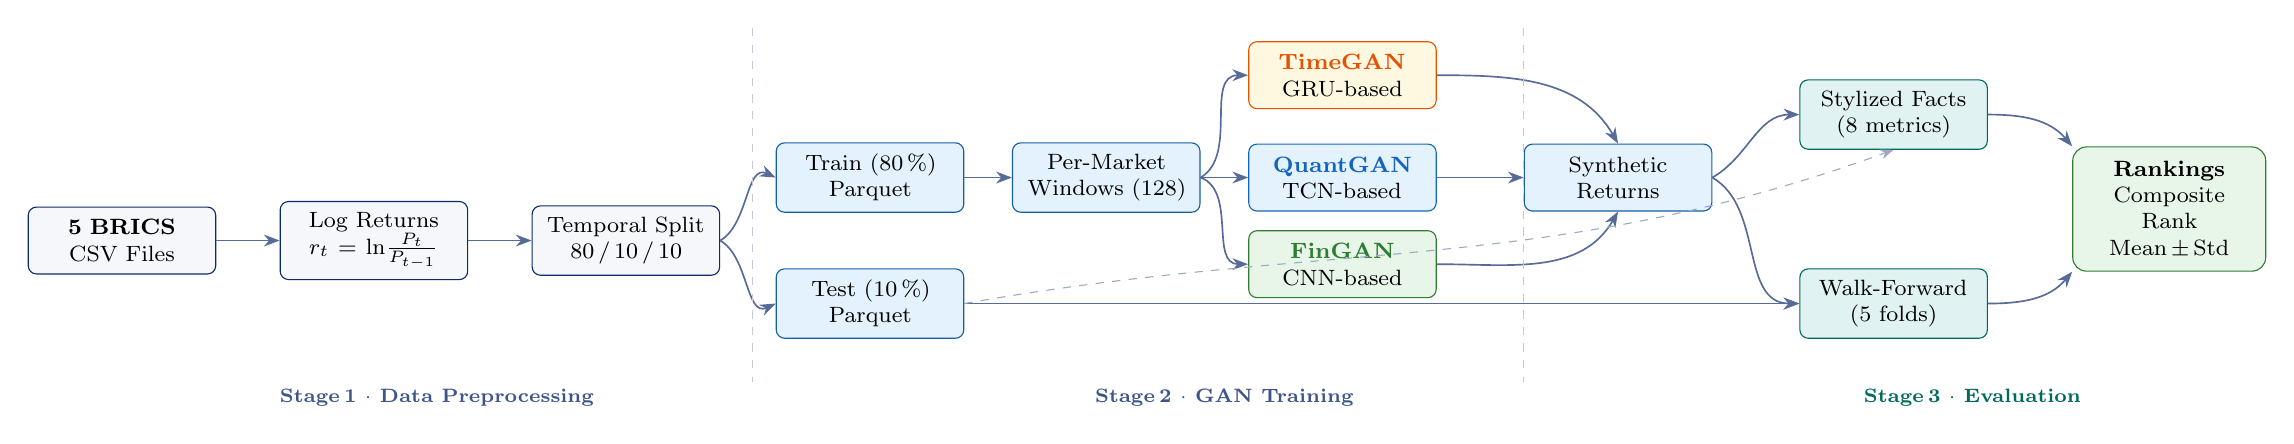
\begin{tikzpicture}[
  every node/.style={font=\footnotesize},
  pp/.style={rectangle, rounded corners=3pt, draw=Navy, fill=LBg,
             text width=2.1cm, align=center, minimum height=0.85cm, inner sep=4pt},
  sp/.style={rectangle, rounded corners=3pt, draw=Sky!80!black, fill=BBg,
             text width=2.1cm, align=center, minimum height=0.85cm, inner sep=4pt},
  ev/.style={rectangle, rounded corners=3pt, draw=Teal, fill=TealBg,
             text width=2.1cm, align=center, minimum height=0.85cm, inner sep=4pt},
  rk/.style={rectangle, rounded corners=5pt, draw=FGreen, fill=GBg,
             text width=2.1cm, align=center, minimum height=1.1cm, inner sep=5pt},
  arr/.style={-Stealth, semithick, draw=Navy!70},
  sarr/.style={-Stealth, thin, draw=Navy!40, dashed},
]

%% ─ Preprocessing nodes ──────────────────────────────────────────────────────
\node[pp] (csv)  at (0.0,  0.0) {\textbf{5 BRICS}\\CSV Files};
\node[pp] (lr)   at (3.2,  0.0) {Log Returns\\$r_t=\ln\!\tfrac{P_t}{P_{t-1}}$};
\node[pp] (spl)  at (6.4,  0.0) {Temporal Split\\80\,/\,10\,/\,10};
\node[sp] (trn)  at (9.5,  0.8) {Train (80\,\%)\\Parquet};
\node[sp] (tst)  at (9.5, -0.8) {Test (10\,\%)\\Parquet};

%% ─ Training nodes ───────────────────────────────────────────────────────────
\node[sp] (poo)  at (12.5,  0.8) {Per-Market\\Windows (128)};

\node[rectangle,rounded corners=3pt,draw=TGcol,fill=ABg,
      text width=2.1cm,align=center,minimum height=0.85cm,inner sep=4pt]
     (tga) at (15.5,  2.1) {\textcolor{TGcol}{\bfseries TimeGAN}\\GRU-based};
\node[rectangle,rounded corners=3pt,draw=QGcol,fill=BBg,
      text width=2.1cm,align=center,minimum height=0.85cm,inner sep=4pt]
     (qga) at (15.5,  0.8) {\textcolor{QGcol}{\bfseries QuantGAN}\\TCN-based};
\node[rectangle,rounded corners=3pt,draw=FGcol,fill=GBg,
      text width=2.1cm,align=center,minimum height=0.85cm,inner sep=4pt]
     (fga) at (15.5, -0.3) {\textcolor{FGcol}{\bfseries FinGAN}\\CNN-based};

%% ─ Evaluation nodes ─────────────────────────────────────────────────────────
\node[sp] (syn)  at (19.0,  0.8) {Synthetic\\Returns};
\node[ev] (sfm)  at (22.5,  1.6) {Stylized Facts\\(8 metrics)};
\node[ev] (wfv)  at (22.5, -0.8) {Walk-Forward\\(5 folds)};
\node[rk] (rnk)  at (26.0,  0.4) {\textbf{Rankings}\\Composite Rank\\Mean\,$\pm$\,Std};

%% ─ Arrows: Preprocessing ────────────────────────────────────────────────────
\draw[arr] (csv.east) -- (lr.west);
\draw[arr] (lr.east)  -- (spl.west);
\draw[arr] (spl.east) to[out= 30,in=155] (trn.west);
\draw[arr] (spl.east) to[out=-30,in=205] (tst.west);

%% ─ Arrows: Training ─────────────────────────────────────────────────────────
\draw[arr] (trn.east) -- (poo.west);
\draw[arr] (poo.east) to[out= 30,in=180] (tga.west);
\draw[arr] (poo.east) --                 (qga.west);
\draw[arr] (poo.east) to[out=-20,in=180] (fga.west);

%% ─ Arrows: Synthesis ────────────────────────────────────────────────────────
\draw[arr] (tga.east) to[out=  0,in=120] (syn.north);
\draw[arr] (qga.east) --                 (syn.west);
\draw[arr] (fga.east) to[out=  0,in=240] (syn.south);

%% ─ Arrows: Evaluation ───────────────────────────────────────────────────────
\draw[arr]  (syn.east) to[out= 30,in=180] (sfm.west);
\draw[arr]  (syn.east) to[out=-30,in=180] (wfv.west);
\draw[arr]  (tst.east) --                 (wfv.west);  %% horizontal; passes below fga
\draw[sarr] (tst.east) to[out=10,in=200]  (sfm.south); %% dashed: test data also into metrics

%% ─ Arrows: Results ──────────────────────────────────────────────────────────
\draw[arr] (sfm.east) to[out=0,in=130] (rnk.north west);
\draw[arr] (wfv.east) to[out=0,in=230] (rnk.south west);

%% ─ Stage labels ─────────────────────────────────────────────────────────────
\node[font=\scriptsize\bfseries,text=Navy!80]  at ( 4.0,-2.0) {Stage\,1 $\cdot$ Data Preprocessing};
\node[font=\scriptsize\bfseries,text=Navy!80]  at (14.0,-2.0) {Stage\,2 $\cdot$ GAN Training};
\node[font=\scriptsize\bfseries,text=Teal]     at (23.5,-2.0) {Stage\,3 $\cdot$ Evaluation};

%% ─ Stage dividers ───────────────────────────────────────────────────────────
\draw[very thin,dashed,Navy!25] ( 8.0, 2.7) -- ( 8.0,-1.8);
\draw[very thin,dashed,Navy!25] (17.8, 2.7) -- (17.8,-1.8);

\end{tikzpicture}
}
\end{center}

\vspace{6pt}
\begin{multicols}{2}

\navybox{What Each Stage Does}{%
\textbf{Stage 1 — Preprocessing:}\ Raw price CSVs are converted to daily log returns
$r_t = \ln(P_t/P_{t-1})$ (stationary, mean-reverting). A strict temporal 80/10/10 split ensures no future data leaks into training. Saved as Parquet (fast columnar I/O).

\smallskip
\textbf{Stage 2 — Training:}\ Each 80\,\% training file is sliced into 128-step sliding windows. Three GAN families are each trained \emph{independently per market} (15 models total: 3 GANs $\times$ 5 markets). No cross-market data is ever mixed, so each model captures only its own market's stylized facts.

\smallskip
\textbf{Stage 3 — Evaluation:}\ Generated synthetic series are compared with real test-set returns on 16 stylized-fact metrics, split into Fidelity (9) and Temporal (7) families (see pages 10a--10c). Walk-forward re-trains each model on 5 rolling folds to verify temporal robustness. Final output: fidelity\_rank, temporal\_rank, composite\_rank, and fold-level mean\,$\pm$\,std.}

\skybox{What Makes This Pipeline Scientifically Novel}{%
\begin{enumerate}
  \item \textbf{Per-market training} --- 15 independent models (3 GANs $\times$ 5 markets) trained with zero cross-market data mixing. This enables per-market analysis and mechanistic explanations (e.g.\ why QuantGAN's TCN better captures Shanghai's long-memory structure), and avoids artificial temporal transitions that would bias stylized-fact metrics.
  \item \textbf{BRICS focus} --- virtually all published GAN-finance benchmarks use S\&P~500 or DAX. BRICS have systematically fatter tails, capital controls (China), and currency effects --- a substantially harder task.
  \item \textbf{No clipping} --- the pipeline preserves extreme returns, which are the defining feature of emerging markets. Adams et al.\ (2019)\tcite{6} show trimming worsens distributional misfit.
  \item \textbf{Walk-forward evaluation} --- single train/test splits give one data point. Rolling-origin evaluation (CTBench 2025\tcite{16}) gives 5, enabling confidence intervals on metric scores.
  \item \textbf{Stylized-fact-first evaluation} --- most published benchmarks use MSE. This pipeline uses 16 financially meaningful metrics (9 Fidelity + 7 Temporal), with a shuffled-control audit that identified 9 permutation-invariant metrics and prompted a two-family composite design.
\end{enumerate}}

\columnbreak

\greenbox{Why BRICS? The Scientific Motivation}{%
\textbf{Risk management gap:}\ global portfolio managers increasingly hold BRICS equities for diversification. Stress-testing these portfolios requires synthetic BRICS scenarios --- but no validated GAN benchmark exists for these markets.

\smallskip
\textbf{Fat-tail severity:}\ BRICS indices have excess kurtosis 2--5$\times$ higher than developed-market equivalents. LeBaron's\tcite{33} EVT work shows their tail indices are lighter ($\alpha \approx 2$--$3$) than the $\alpha \approx 3$--$4$ typical in the US. A synthetic-data generator trained on S\&P~500 data would \emph{underestimate} these tails.

\smallskip
\textbf{Data scarcity:}\ BRICS markets have shorter histories ($\approx$25 years for Chinese A-shares vs $100+$ years for S\&P~500). GAN augmentation is therefore more valuable here than for developed markets.}

\redbox{Why This Study Is Publishable: The Journal Pitch}{%
\textbf{Gap:} as of 2025, no paper systematically compares GAN architectures specifically on BRICS emerging-market log returns with CTBench-compliant evaluation.

\textbf{Contribution 1:}\ First multi-architecture GAN benchmark (TimeGAN + QuantGAN + FinGAN) on BRICS emerging-market data with per-market training and walk-forward temporal validation --- 15 models, 5 markets, 16 stylized-fact metrics (9 Fidelity + 7 Temporal).

\textbf{Contribution 2:}\ Full stylized-fact evaluation using the CTBench metric set (energy distance, discriminative AUC, Hurst exponent, ARCH-LM), replacing the naive MSE used in most prior work.

\textbf{Contribution 3:}\ A reproducible pipeline (seeded, code-released) with explicit methodology for handling emerging-market tail events (no clipping, EVT-motivated evaluation).

\textbf{Target journals:}\ \textit{Quantitative Finance} (Taylor \& Francis); \textit{Journal of Financial Economics}; \textit{Finance Research Letters}.}

\end{multicols}

\clearpage

%% ─── Page 15: GAN Fundamentals — Feynman Style ──────────────────────────────
\pagehead{Knowledge Base I --- GAN Fundamentals (Explained from First Principles)}
         {Target reader: calculus 1 background, no prior machine learning knowledge}

\begin{multicols}{2}

\navybox{What is a Generative Model?}{%
\textbf{In one sentence:}\ a generative model learns the distribution of real data and can then \emph{draw new samples} that look statistically identical to the training set.

\smallskip
\textbf{Everyday analogy:}\ imagine a music teacher who has heard 10\,000 piano pieces. After enough listening, they can compose new pieces that ``sound right'' --- same key signatures, same chord progressions, same dynamic patterns --- even though no individual piece was memorised.

\smallskip
\textbf{In finance:}\ a generative model for daily log returns learns ``what a realistic market day looks like'': how volatile, how skewed, how correlated with yesterday. It can then produce as many synthetic trading days as you need.

\smallskip
\textbf{How it's represented mathematically:}\ the model is a function $G(z)$ that takes random noise $z \sim \mathcal{N}(0,I)$ as input and outputs a fake sample $\tilde{x} = G(z)$. Training adjusts $G$'s parameters so that the distribution of $\tilde{x}$ matches the distribution of real data $x$.}

\skybox{The GAN: Two AIs Competing}{%
\textbf{In one sentence:}\ a GAN trains a Generator (G) and a Discriminator (D) simultaneously; G tries to fool D, D tries to catch G, and each improves by losing to the other.

\smallskip
\textbf{The counterfeiter analogy:}
\begin{itemize}
  \item \textbf{Generator (G)} = a counterfeiter printing fake bank notes.
  \item \textbf{Discriminator (D)} = a bank detective checking each note.
  \item G submits fake notes. D marks them FAKE or REAL.
  \item G improves by studying why its fakes were rejected.
  \item D improves by finding subtler distinguishing features.
  \item After enough rounds: G's fakes are indistinguishable from real notes. Game over.
\end{itemize}
This was proposed by Goodfellow et al.\ (2014, NeurIPS)\tcite{1} and is the foundation for TimeGAN, QuantGAN, and FinGAN.}

\tealbox{The Math of the Competition (Minimax Game)}{%
G minimises, D maximises the same objective $V(G,D)$:
\begin{align*}
\min_G \max_D V(G,D) &=
  \underbrace{\E_{x\sim p_\text{data}}[\log D(x)]}_\text{D rewarded for calling real ``real''} \\
  &+\underbrace{\E_{z\sim p_z}[\log(1-D(G(z)))]}_\text{D rewarded for calling fake ``fake''}
\end{align*}
\textbf{Calculus 1 connection:}\ $V$ is just a function of the parameters $\theta_G$ and $\theta_D$. Training = gradient descent for G (minimise) and gradient ascent for D (maximise). The derivative $\partial V / \partial \theta_G$ tells G which direction to move to fool D.

\textbf{Ideal outcome:}\ $D(x) = 0.5$ everywhere --- D cannot do better than random guessing because real and fake are perfectly mixed.}

\columnbreak

\amberbox{Why Plain GANs Fail on Financial Data}{%
\textbf{Problem 1 --- Mode collapse:}\ G finds ONE output that always fools D and produces only that output forever. Instead of generating the full range of market scenarios, it only generates one type (e.g., always very calm days). G's loss goes to zero but its outputs are useless.

\smallskip
\textbf{Problem 2 --- Discriminator saturation:}\ early in training, D easily spots fakes (the generator hasn't learned yet). The sigmoid output $D(G(z)) \approx 0$, and $\log(1-D(G(z))) \approx 0$ (saturated). The gradient flowing back to G is nearly zero --- G cannot learn from a perfect discriminator.

\smallskip
\textbf{Problem 3 --- No guarantee of convergence:}\ the min-max game can cycle rather than converge. The discriminator and generator take turns ``winning'', never reaching a stable equilibrium.

\smallskip
\textbf{Problem 4 --- Temporal structure lost:}\ a vanilla GAN treats each output position independently, without enforcing that consecutive returns follow the volatility-clustering and long-memory patterns of real markets.}

\redbox{Fix 1 --- The Wasserstein GAN (WGAN)}{%
\textbf{In one sentence:}\ instead of asking ``real or fake?'' (binary classification), WGAN asks ``how different are the two distributions?'' using the Wasserstein (Earth-Mover) distance.

\smallskip
\textbf{Earth-mover analogy:}\ imagine the real distribution and fake distribution as two piles of dirt. The Wasserstein distance is the minimum total effort to move one pile to match the other: (weight of dirt) $\times$ (distance moved), summed over all dirt.
\begin{equation*}
  W(p,q) = \inf_{\gamma \in \Pi(p,q)} \E_{(x,y)\sim\gamma}\|x-y\|
\end{equation*}

\textbf{Why it fixes saturation:}\ the Wasserstein distance has a meaningful gradient even when the two distributions have no overlap. The critic (D in WGAN) always provides a useful learning signal, even at the very start of training when the generator is terrible (Arjovsky et al., 2017, ICML).}

\purplebox{Fix 2 --- Gradient Penalty (WGAN-GP)}{%
\textbf{The Lipschitz constraint:}\ Wasserstein distance requires the critic $D$ to be ``1-Lipschitz'': its output cannot change faster than 1 unit per unit of input change. Think of it as requiring the critic to be \emph{consistent} --- similar inputs get similar scores.

\smallskip
\textbf{The penalty:}\ instead of hard constraints (weight clipping, which causes gradient explosion), Gulrajani et al.\ (2017, NeurIPS)\tcite{3} add a soft penalty to the training loss:
\begin{equation*}
  \mathcal{L}_\text{GP} = \lambda \cdot \E_{\hat{x}}
  \bigl[(\|\nabla_{\hat{x}}D(\hat{x})\|_2 - 1)^2\bigr]
\end{equation*}
where $\hat{x}$ is a random mixture of real and fake. If the gradient norm deviates from 1, the critic is penalised. \textbf{Fixed values:} $\lambda=10$, $n_\text{critic}=5$ (the critic is updated 5 times per generator step). These are not hyperparameters to search over --- they are literature-anchored constants.}

\end{multicols}

\clearpage

%% ─── Page 16: Neural Network Building Blocks ────────────────────────────────
\pagehead{Knowledge Base II --- Neural Network Components Explained}
         {GRU $\cdot$ Conv1d $\cdot$ TCN $\cdot$ ConvTranspose1d $\cdot$ LayerNorm $\cdot$ Adam $\cdot$ seq\_len}

\begin{multicols}{2}

\navybox{What is a Neural Network? (Calculus 1 Perspective)}{%
\textbf{In one sentence:}\ a neural network is a very complicated function with millions of adjustable parameters, organised in layers, that can approximate any pattern if given enough parameters and training examples.

\smallskip
\textbf{Calculus 1 version:}\ you already know how to minimise $f(x) = x^2$: take the derivative $f'(x)=2x$, set it to zero. A neural network minimises a loss function $\mathcal{L}(\theta)$ over millions of parameters $\theta$ using the same idea: repeatedly subtract a small multiple of the gradient $\nabla_\theta \mathcal{L}$:
\[\theta \leftarrow \theta - \alpha \nabla_\theta \mathcal{L}(\theta)\]
This is called \textbf{gradient descent}. The gradient $\nabla_\theta \mathcal{L}$ is computed by the chain rule (Calculus 1: derivative of a composed function). Called \textbf{backpropagation} in neural-network literature.}

\skybox{The Vanishing Gradient Problem}{%
\textbf{In one sentence:}\ in a deep network, the gradient signal shrinks exponentially as it travels backward through layers, leaving early layers unable to learn.

\smallskip
\textbf{The chain rule:}\ for a 50-layer network, the chain rule gives:
\[\frac{\partial \mathcal{L}}{\partial w_1} = \frac{\partial \mathcal{L}}{\partial h_{50}} \cdot \frac{\partial h_{50}}{\partial h_{49}} \cdots \frac{\partial h_2}{\partial h_1} \cdot \frac{\partial h_1}{\partial w_1}\]
Each $\frac{\partial h_{i+1}}{\partial h_i} \approx 0.5$ in a typical network. After 50 layers: $0.5^{50} \approx 10^{-15}$. Essentially zero. Layer 1 gets no useful gradient.

\smallskip
\textbf{Relevance here:}\ (1) GRU cells solve this for the time dimension via gating. (2) WGAN-GP provides well-behaved gradients to the generator even when distributions are far apart, avoiding the saturation-to-zero problem of the standard GAN loss.}

\tealbox{Adam: The Smart Optimizer}{%
\textbf{In one sentence:}\ Adam adjusts the step size differently for each parameter, taking small steps in directions you've been inconsistent and large steps in directions you've been consistent.

\smallskip
\textbf{Hiking analogy:}\ imagine hiking in fog. Where you've stumbled a lot (high past gradient variance), take small careful steps. Where you've been walking steadily in one direction, stride longer. Adam keeps track of both the average gradient (momentum, $\beta_1$) and the average squared gradient (variance, $\beta_2$) per parameter.

\smallskip
$\beta_1 = 0$ for WGAN-GP: In adversarial training, the correct direction for the generator changes every step (because the critic updates between each generator step). Momentum would carry old, now-wrong information. Setting $\beta_1=0$ uses only the \emph{current} gradient. $\beta_2=0.9$ is standard for all models (Gulrajani et al., 2017).}

\greenbox{seq\_len: What Counts as One Training Example?}{%
\textbf{In one sentence:}\ the model processes the time series as fixed-length windows of \texttt{seq\_len=128} consecutive days; each window is one training example.

\smallskip
\textbf{Why 128?}\ Long enough to capture volatility clustering (which persists for days to weeks), short enough to create thousands of overlapping training examples from a 5-year dataset.

\smallskip
\textbf{Sliding window:}\ from a 1\,000-day series we get 1\,000\,$-$\,128\,$+$\,1\,$=$\,873 windows. Each market's 80\,\% training split ($\approx$800 days) yields $\approx$673 windows --- enough to learn distributional patterns. Models train on one market's windows only; no cross-market data is mixed.

\smallskip
\textbf{FinGAN constraint:}\ \texttt{seq\_len} must be divisible by 8. Three \texttt{ConvTranspose1d} layers each double the length ($2^3=8$); FinGAN starts from noise of length $\texttt{seq\_len}/8$ and expands to \texttt{seq\_len}.}

\columnbreak

\navybox{GRU: Memory Cells for Sequential Data (TimeGAN)}{%
\textbf{In one sentence:}\ a GRU (Gated Recurrent Unit, Cho et al.\ 2014)\tcite{19} is a mathematical ``memory'' that reads a sequence one step at a time and decides at each step what to remember and what to forget.

\smallskip
\textbf{The gate analogy:}\ imagine reading market news one headline at a time. At each new headline you make two decisions: (1) \textbf{Update gate} $z_t$: is this headline important enough to UPDATE my view? (2) \textbf{Reset gate} $r_t$: should I FORGET my past view before reading this?
\[h_t = (1-z_t)\cdot h_{t-1} + z_t \cdot \tilde{h}_t, \quad z_t = \sigma(W_z[h_{t-1},x_t])\]
$h_t$ is the GRU's ``memory'' (hidden state). The sigmoid $\sigma$ makes the gate a smooth 0-to-1 switch.

\smallskip
\textbf{Why GRU in TimeGAN:}\ financial volatility clustering spans days to weeks. GRU maintains context across these time scales without vanishing gradients (the gates prevent gradient shrinkage). Yoon et al.\ (2019)\tcite{4} validated GRU as the backbone for sequential GAN training at NeurIPS.}

\skybox{Conv1d + TCN: Pattern Detection at Multiple Scales (QuantGAN)}{%
\textbf{Conv1d in one sentence:}\ slide a small learned ``pattern template'' (kernel) along the time series; the output is a score for how well the template matches each position.

\smallskip
\textbf{Analogy:}\ a spell-checker slides a window of 5 characters across a document, checking for known misspelling patterns. Similarly, a Conv1d kernel of length 5 slides over 128 days of returns, scoring each 5-day window on a learned pattern (e.g., reversal, momentum spike).

\smallskip
\textbf{TCN (Temporal Convolutional Network):}\ stacks Conv1d layers but with \emph{exponentially growing gaps} (dilations). Layer 1 looks at today $\pm$1 day. Layer 2 at today $\pm$2 days. Layer 3 at today $\pm$4 days. After 7 layers: receptive field covers 127 days --- the entire window --- with only 7 layers worth of parameters (Bai et al., 2018\tcite{20}, arXiv\tcite{20}).

\smallskip
\textbf{Why QuantGAN uses TCN:}\ multi-scale financial patterns (intraday microstructure, weekly seasonality, monthly cycles) require exactly this hierarchical temporal coverage. Wiese et al.\ (2020, \textit{Quantitative Finance})\tcite{5} showed TCN+WGAN-GP outperforms RNN-based generators on Hurst exponent fidelity.}

\amberbox{ConvTranspose1d: The Expanding Generator (FinGAN)}{%
\textbf{In one sentence:}\ ConvTranspose1d is the \emph{reverse} of Conv1d --- instead of compressing a long signal into fewer values, it \emph{expands} a short vector into a longer sequence.

\smallskip
\textbf{Video upscaling analogy:}\ a 32-pixel image scaled to 96 pixels --- each output pixel is a weighted sum of nearby input pixels, but the weights ``spread'' information outward. ConvTranspose1d does the same in 1D.

\smallskip
\textbf{FinGAN's Generator:}\ takes noise $z$ of length 16 $\to$ ConvTranspose1d $\to$ length 32 $\to$ ConvTranspose1d $\to$ length 64 $\to$ ConvTranspose1d $\to$ length 128 (= \texttt{seq\_len}). Each step doubles the length and halves the ``abstraction''. The model learns to produce realistic return sequences from random seeds.}

\indigobox{LayerNorm: Keeping Values Calibrated}{%
\textbf{In one sentence:}\ for each sample \emph{independently}, subtract its mean and divide by its standard deviation before passing to the next layer --- keeps activations in a stable numerical range.

\smallskip
\textbf{Calibration analogy:}\ grading multiple exams, some scored 0--10, others 0--100. Before comparing, rescale each exam to a 0--1 range. LayerNorm does this for each neural network ``sample'' individually.

\smallskip
\textbf{Why not BatchNorm?}\ BatchNorm normalises \emph{across} the batch (all samples together). With small batches (32--64 samples), batch statistics are noisy, causing unstable GAN training. LayerNorm normalises \emph{within} each sample, independent of batch size.

\smallskip
\textbf{In FinGAN's Critic:}\ the critic receives both real returns (say, scale 0.01--0.03 std) and early-training fakes (scale 0.5--5.0 std). LayerNorm prevents the critic from using scale alone to distinguish them --- forcing it to learn distributional \emph{shape} differences instead.}

\end{multicols}

\clearpage

%% ─── Page 17: The Three Architectures Compared ──────────────────────────────
\pagehead{Knowledge Base III --- TimeGAN, QuantGAN, and FinGAN Side by Side}
         {What each architecture assumes about financial time series, and why}

\vspace{4pt}
{\small
\begin{tabularx}{\linewidth}{@{}lXXX@{}}
\toprule
 & \textbf{\textcolor{TGcol}{TimeGAN}} & \textbf{\textcolor{QGcol}{QuantGAN}} & \textbf{\textcolor{FGcol}{FinGAN}} \\
\midrule
\textbf{Core architecture} & 4-phase (encoder + supervisor + GAN) using GRU & TCN-based WGAN-GP & CNN deconvolution WGAN-GP \\
\textbf{Temporal mechanism} & Recurrent (GRU): processes each step in order & Dilated convolutions: parallel look at all scales & Transposed convolutions: upsamples from short to long \\
\textbf{Training method} & BCE + moment-matching loss; 4 separate training phases & WGAN-GP (single phase) & WGAN-GP (single phase) \\
\textbf{Literature reference} & Yoon et al.\ (2019, NeurIPS)\tcite{4} & Wiese et al.\ (2020, \textit{Quant.\ Finance})\tcite{5} & Custom (this paper) \\
\textbf{Key hyperparameters} & hidden\_dim, num\_layers, lr & lr, noise\_dim (n\_critic=5 fixed) & lr, noise\_dim (n\_critic=5 fixed) \\
\textbf{seq\_len constraint} & Any length & Any length & Must be divisible by 8 \\
\textbf{Inductive bias} & Temporal ordering matters step-by-step & Multi-scale patterns (short+long memory) & Generate from compressed noise, like image GANs \\
\textbf{BRICS hypothesis} & GRU memory captures volatility regime persistence & Dilations capture BRICS multi-scale clustering & Deconv captures heavy-tail shape from noise \\
\bottomrule
\end{tabularx}}

\vspace{6pt}
\begin{multicols}{2}

\navybox{TimeGAN: Four Phases to Learn Temporal Structure}{%
Yoon et al.\ (2019)\tcite{4} recognised that a plain GAN ignores the \emph{order} of time steps. Their solution: embed data into a learned latent space first, then generate in that space.

\smallskip
\textbf{Phase 1 --- Autoencoder:}\ train an Encoder ($E$) and Recovery ($R$) so that $R(E(x)) \approx x$. This builds a compressed ``language'' the GAN will speak. Like learning music notation before composing.

\textbf{Phase 2 --- Supervisor:}\ train a Supervisor ($S$) that predicts the \emph{next} latent step $h_{t+1}$ from the current one $h_t$. This injects temporal causality into the model.

\textbf{Phase 3 --- Joint GAN:}\ train G and D simultaneously in the latent space, with the supervisor providing an extra loss term $\mathcal{L}_\text{S} = \|h_{t+1} - S(h_t)\|^2$ (moment matching).

\textbf{Phase 4 --- Refinement:}\ fine-tune the recovery $R$ with generated latent sequences. Final output: $\tilde{x} = R(G(z))$.

\textbf{Limitation here:}\ \texttt{epochs=5} means each phase gets $\sim$2 gradient steps. TimeGAN's GRU cannot converge in 2 steps (Yoon et al.\ used 5\,000--10\,000 iterations per phase). \textcolor{DRed}{\textbf{This is the most critical open bug.}}}

\skybox{QuantGAN: Dilated Patterns Across Time Scales}{%
Wiese et al.\ (2020)\tcite{5} adapted the WGAN-GP framework to financial time series by replacing the usual MLP with a Temporal Convolutional Network (TCN).

\smallskip
\textbf{Generator $G$:}\ noise $z$ of length \texttt{seq\_len} $\to$ stack of dilated Conv1d layers $\to$ synthetic returns. Each layer's dilation doubles ($d = 1, 2, 4, 8, \ldots$), so layer $k$ sees the entire context with only $2^k$ effective lags.

\textbf{Critic $D$:}\ same TCN structure, but maps sequences to a single scalar (``how real is this?''). WGAN-GP training: critic updated $n_\text{critic}=5$ times per generator step.

\textbf{Why this works for BRICS:}\ volatility clustering in BRICS markets operates simultaneously at intraday, weekly, and monthly time scales. Dilated convolutions cover all three scales in a single forward pass. Wiese et al.\ showed this architecture reproduces the Hurst exponent of equity returns significantly better than LSTM-based generators.}

\columnbreak

\tealbox{FinGAN: Generating Sequences like Images}{%
FinGAN borrows from image generation (Radford et al., DCGAN 2015)\tcite{21} and applies it to 1-D financial sequences.

\smallskip
\textbf{Generator $G$:}\ noise $z$ (dimension 100) $\xrightarrow{\text{FC}}$ tensor of shape (64, 16) $\xrightarrow{\text{ConvT1d}\times 3}$ (1, 128). Each ConvTranspose1d doubles the temporal length ($16 \to 32 \to 64 \to 128$) while reducing channels (64 $\to$ 32 $\to$ 16 $\to$ 1).

\textbf{Critic $D$:}\ mirrors G in reverse. Sequence (1, 128) $\xrightarrow{\text{Conv1d}\times 3}$ features (64, 16) $\to$ scalar. LayerNorm after each Conv1d stabilises training.

\textbf{Inductive bias:}\ deconvolution builds long sequences from hierarchical abstractions, the same way an image GAN builds textures from abstract ``concepts''. For finance, this means the model first decides the broad return regime (high/low volatility) and then fills in fine-grained daily fluctuations.

\textbf{Novelty:}\ no prior paper applies CNN deconvolution WGAN-GP to BRICS markets with explicit stylized-fact evaluation. This is a direct contribution of the current study.}

\greenbox{Why Compare All Three? The Inductive Bias Argument}{%
Each architecture encodes a different prior belief about how financial time series work:
\begin{itemize}
  \item \textbf{TimeGAN (GRU)}: ``returns are causally ordered; today's volatility is a function of recent history.'' This is the textbook financial econometrics view.
  \item \textbf{QuantGAN (TCN)}: ``volatility operates at multiple time scales simultaneously.'' This aligns with multi-fractal market models.
  \item \textbf{FinGAN (CNN)}: ``market regimes are hierarchical; fine-grained returns are conditioned on a macro-state.'' This aligns with hidden Markov / regime-switching models.
\end{itemize}
Comparing all three reveals \emph{which structural assumption best describes BRICS markets} --- a theoretically interesting result, not just an engineering comparison. This is the core scientific question the paper answers.}

\end{multicols}

\clearpage

%% ─── Page 18: Evaluation Glossary ───────────────────────────────────────────
\pagehead{Knowledge Base IV --- Complete Evaluation Glossary}
         {Every metric, test, and concept in this report explained in plain language}

\begin{multicols}{2}

\indigobox{ACF / Autocorrelation Function}{%
\textbf{In one sentence:}\ measures how similar a time series is to a shifted copy of itself.

$\rho_k = \text{Corr}(r_t,\, r_{t-k})$. For log returns: $\rho_k \approx 0$ (efficient markets). For $|r_t|$: $\rho_k > 0$ for $k = 1$--$100+$ (volatility clustering). A good GAN reproduces both patterns simultaneously. Our metric: mean absolute error between the real and synthetic ACF curves (ACF MAE).}

\indigobox{ARCH Effects / ARCH-LM Test}{%
\textbf{In one sentence:}\ ARCH effects mean ``the variance of returns today depends on the variance yesterday'' --- volatility comes in clusters.

Named after Robert Engle (1982)\tcite{10}\tcite{10} Nobel Prize). The LM test regresses $\hat{r}_t^2$ on its own lags; a significant $\chi^2$ statistic means ARCH is present. BRICS returns almost always show strong ARCH. A synthetic series that does NOT show ARCH has failed to capture a key stylized fact.}

\indigobox{Discriminative AUC}{%
\textbf{In one sentence:}\ train a simple classifier to tell real from fake; if it can't do better than coin-flipping (AUC = 0.5), the synthetic data is indistinguishable.

\textbf{AUC} (Area Under the ROC Curve) = probability that the classifier ranks a real sample higher than a fake sample. AUC = 1.0 means trivially separable; AUC = 0.5 means perfect indistinguishability. Our implementation: logistic regression on 20-day rolling-window features (mean, std, mean-abs, mean-sq), 5-fold cross-validation. Based on TSGBench (Ang et al., 2023\tcite{15}, PVLDB\tcite{15})\tcite{15}.}

\indigobox{Energy Distance}{%
\textbf{In one sentence:}\ a proper mathematical distance between two distributions, computed from pairwise distances between samples --- robust to serial dependence.

$E(P,Q) = 2\E\|X-Y\| - \E\|X-X'\| - \E\|Y-Y'\|$, where $X,X' \sim P$ (real), $Y,Y' \sim Q$ (synthetic). Székely \& Rizzo (2004). $E \geq 0$; $E=0 \Leftrightarrow P=Q$. Unlike KS p-values, the energy distance is interpretable even with serially correlated data, because it doesn't assume i.i.d.\ samples.}

\indigobox{Hurst Exponent ($H$)}{%
\textbf{In one sentence:}\ measures how ``trendy'' a time series is; $H > 0.5$ means past moves predict future moves.

Estimated via the R/S (Rescaled Range) method applied to \emph{absolute returns} $|r_t|$:
$\E[R_n/S_n] \sim c \cdot n^H$. For $H=0.5$: random walk (Brownian motion). For $H > 0.5$: long memory --- large $|r|$ today predicts large $|r|$ tomorrow. Typical daily $|r_t|$: $H \approx 0.6$--$0.7$ (Ding et al., 1993\tcite{8}).

\textbf{Debate:}\ rough-volatility theory (Gatheral et al., 2018) estimates $H \approx 0.1$ on intraday \emph{realised variance} using a different estimator at a different time scale --- both camps can be correct simultaneously (Cont \& Das, 2024\tcite{18}). Our metric: $|H_\text{real} - H_\text{syn}|$ on daily $|r_t|$ via R/S.}

\indigobox{KS Test (Kolmogorov-Smirnov)}{%
\textbf{In one sentence:}\ tests whether two samples could plausibly come from the same distribution, using the maximum gap between their empirical CDFs.

$D = \max_x |F_n(x) - G_m(x)|$. Under $H_0$ (same distribution), the p-value should be uniform on [0,1]. \textbf{Limitation:}\ assumes i.i.d.\ samples. Financial returns are serially correlated ($\rho_k \neq 0$ for $|r_t|$), inflating the test statistic and making p-values anti-conservative ($n_\text{eff} = n/11$ to $n/31$). Retained in the report with caveat; not used as the primary metric.}

\columnbreak

\indigobox{Quantile MSE (QMSE)}{%
\textbf{In one sentence:}\ compare the $k$-th smallest real return to the $k$-th smallest synthetic return, for $k = 1\%$ to $99\%$ of the sorted series.
\[\text{QMSE} = \frac{1}{K}\sum_{k=1}^K (Q_\text{real}(\alpha_k) - Q_\text{syn}(\alpha_k))^2\]
This is the only sensible ``pointwise'' comparison between two unaligned distributions --- comparing by rank, not by date. A large QMSE at the tails (1\%, 5\%, 95\%, 99\%) means the GAN misses extreme events. Equivalent to the $L^2$ distance between empirical CDFs.}

\indigobox{Tail Index (Hill Estimator)}{%
\textbf{In one sentence:}\ measures how ``extreme'' the extreme events are; lower tail index = heavier tail = more frequent crashes/spikes.

The Hill estimator: sort $|r_t|$ in ascending order; take the largest $k$ values; $\hat{\alpha} = k / \sum \log(|r|_{(n-i)}/|r|_{(n-k)})$. For a normal distribution: $\alpha = \infty$ (no power-law tail). For financial returns: $\alpha \approx 2$--$4$ (Pareto-like tails). Lower $\alpha$ in BRICS vs developed markets is why BRICS are a more interesting test case.}

\indigobox{Volatility Clustering}{%
\textbf{In one sentence:}\ large price moves tend to be followed by large moves (regardless of direction), and small moves by small moves.

Mathematically: $|\text{Corr}(|r_t|, |r_{t+k}|)| > 0$ for $k = 1, 2, \ldots, 100$. This is NOT saying direction repeats (that would violate market efficiency); only that \emph{magnitude} repeats. Mandelbrot (1963)\tcite{9} observed this first. Our metric: ACF MAE on $|r_t|$ and $r_t^2$.}

\indigobox{Walk-Forward Validation}{%
\textbf{In one sentence:}\ instead of one train/test split, roll the training window forward 5 times and report the mean and standard deviation of results across folds.

\textbf{Why:}\ a single train/test split gives exactly one metric score. Is this score lucky or representative? Walk-forward gives 5 scores, enabling mean\,$\pm$\,std --- the standard robustness evidence required for time-series papers (Tashman 2000\tcite{13}; Bergmeir \& Ben\'{\i}tez 2012\tcite{14}). Our implementation: 5 folds per market, model retrained from scratch each fold on that market's own test series --- no cross-market mixing.}

\indigobox{Wasserstein Distance}{%
\textbf{In one sentence:}\ the minimum work needed to rearrange the fake distribution into the real one, where ``work'' = mass × distance moved.

$W_1(p,q) = \inf_\gamma \E_{(x,y) \sim \gamma}\|x-y\|$ where $\gamma$ is any joint distribution with marginals $p$ and $q$. The Kantorovich-Rubinstein duality makes this tractable: $W_1(p,q) = \sup_{\|f\|_L \leq 1}(\E_p[f] - \E_q[f])$. WGAN-GP trains the critic $f$ to be the optimal 1-Lipschitz function. Our metric: empirical Wasserstein-1 (implemented by \texttt{scipy.stats.wasserstein\_distance}).}

\indigobox{The 10 Stylized Facts in Plain Language}{%
\begin{enumerate}[leftmargin=12pt]
  \item \textbf{Fat tails:}\ extreme returns happen far more often than Gaussian.
  \item \textbf{Near-zero ACF:}\ today's return direction doesn't predict tomorrow's direction.
  \item \textbf{Volatility clustering:}\ today's \emph{magnitude} \emph{does} predict tomorrow's magnitude.
  \item \textbf{Long memory:}\ the ACF of $|r_t|$ decays slowly (weeks to months).
  \item \textbf{Negative skewness:}\ crashes are faster and sharper than rallies.
  \item \textbf{Leverage effect:}\ drops in price → increases in volatility (asymmetric).
  \item \textbf{Gain/loss asymmetry:}\ losses cluster more tightly than gains.
  \item \textbf{ARCH effects:}\ conditional variance is predictable (Engle, 1982\tcite{10}).
  \item \textbf{Extreme events:}\ returns beyond $2\sigma$ occur $>$5\,\% of days (vs 4.6\,\% Gaussian).
  \item \textbf{Distributional match:}\ full CDF shape, not just first 4 moments.
\end{enumerate}
A GAN that reproduces all 10 is considered finance-grade. None of the three tested models perfectly reproduces all 10 on BRICS data.}

\end{multicols}



%% ─────────────────────────────────────────────────────────────────────────────
%% REFERENCES
%% ─────────────────────────────────────────────────────────────────────────────
\clearpage
\phantomsection

% References header — matches report style
\begin{tcolorbox}[
  colback=NavyBg, colframe=NavyBg!60!black, arc=4pt,
  left=8pt, right=8pt, top=4pt, bottom=4pt,
  before skip=0pt, after skip=10pt]
{\large\bfseries\color{Navy} References}
\end{tcolorbox}

{\small
\begin{enumerate}[label={\textbf{[\arabic*]}},leftmargin=2.8em,itemsep=5pt,parsep=0pt,topsep=2pt]

\item \hypertarget{R:1}{}%
  Goodfellow, I., Pouget-Abadie, J., Mirza, M., Xu, B., Warde-Farley, D., Ozair, S., Courville, A., \& Bengio, Y.\ (2014).
  Generative Adversarial Nets.
  \textit{Advances in Neural Information Processing Systems (NeurIPS)}, 27, 2672--2680.

\item \hypertarget{R:2}{}%
  Arjovsky, M., Chintala, S., \& Bottou, L.\ (2017).
  Wasserstein Generative Adversarial Networks.
  \textit{International Conference on Machine Learning (ICML)},
  Proceedings of Machine Learning Research 70, pp.\ 214--223.

\item \hypertarget{R:3}{}%
  Gulrajani, I., Ahmed, F., Arjovsky, M., Dumoulin, V., \& Courville, A.\ (2017).
  Improved Training of Wasserstein GANs.
  \textit{Advances in Neural Information Processing Systems (NeurIPS)}, 30.

\item \hypertarget{R:4}{}%
  Yoon, J., Jarrett, D., \& van der Schaar, M.\ (2019).
  Time-series Generative Adversarial Networks.
  \textit{Advances in Neural Information Processing Systems (NeurIPS)}, 32, 5508--5518.

\item \hypertarget{R:5}{}%
  Wiese, M., Knobloch, R., Korn, R., \& Kretschmer, P.\ (2020).
  Quant GANs: Deep Generation of Financial Time Series.
  \textit{Quantitative Finance}, 20(9), 1419--1440.

\item \hypertarget{R:6}{}%
  Adams, Z., F\"u{\ss}, R., \& Gl\"uck, T.\ (2019).
  Are correlations constant? Empirical and theoretical results on popular distributional
  assumptions in finance.
  \textit{Financial Management}, 48(3), 793--826.

\item \hypertarget{R:7}{}%
  Cont, R.\ (2001).
  Empirical properties of asset returns: stylized facts and statistical issues.
  \textit{Quantitative Finance}, 1(2), 223--236.

\item \hypertarget{R:8}{}%
  Ding, Z., Granger, C.\ W.\ J., \& Engle, R.\ F.\ (1993).
  A long memory property of stock market returns and a new model.
  \textit{Journal of Empirical Finance}, 1(1), 83--106.

\item \hypertarget{R:9}{}%
  Mandelbrot, B.\ (1963).
  The variation of certain speculative prices.
  \textit{The Journal of Business}, 36(4), 394--419.

\item \hypertarget{R:10}{}%
  Engle, R.\ F.\ (1982).
  Autoregressive conditional heteroscedasticity with estimates of the variance of
  United Kingdom inflation.
  \textit{Econometrica}, 50(4), 987--1007.

\item \hypertarget{R:11}{}%
  Sz\'{e}kely, G.\ J., \& Rizzo, M.\ L.\ (2004).
  Testing for equal distributions in high dimension.
  \textit{InterStat}, 5(16.10), 1249--1272.

\item \hypertarget{R:12}{}%
  Bergstra, J., \& Bengio, Y.\ (2012).
  Random search for hyper-parameter optimization.
  \textit{Journal of Machine Learning Research (JMLR)}, 13, 281--305.

\item \hypertarget{R:13}{}%
  Tashman, L.\ J.\ (2000).
  Out-of-sample tests of forecasting accuracy: an analysis and review.
  \textit{International Journal of Forecasting}, 16(4), 437--450.

\item \hypertarget{R:14}{}%
  Bergmeir, C., \& Ben\'{\i}tez, J.\ M.\ (2012).
  On the use of cross-validation for time series predictor evaluation.
  \textit{Information Sciences}, 191, 192--213.

\item \hypertarget{R:15}{}%
  Ang, Y., Bansal, P., Gupta, G., \& Su, L.\ (2023).
  TSGBench: Time Series Generation Benchmark.
  \textit{Proceedings of the VLDB Endowment (PVLDB)}, 17(3), 305--318.

\item \hypertarget{R:16}{}%
  Liao, Q.\ et al.\ (2025).
  CTBench: A Comprehensive and Extensible Benchmark for Conditional Time Series Generation.
  \textit{Advances in Neural Information Processing Systems (NeurIPS)}, 38,
  Datasets and Benchmarks Track.

\item \hypertarget{R:17}{}%
  Gatheral, J., Jaisson, T., \& Rosenbaum, M.\ (2018).
  Volatility is rough.
  \textit{Quantitative Finance}, 18(6), 933--949.

\item \hypertarget{R:18}{}%
  Cont, R., \& Das, S.\ (2024).
  Rough volatility: fact or artefact?
  \textit{Sankhya B}, 86(1), 191--223.

\item \hypertarget{R:19}{}%
  Cho, K., van Merrienboer, B., G\"{u}l\c{c}ehre, \c{C}., Bahdanau, D., Bougares, F.,
  Schwenk, H., \& Bengio, Y.\ (2014).
  Learning phrase representations using RNN encoder--decoder for statistical machine translation.
  \textit{Proceedings of EMNLP 2014}, pp.\ 1724--1734.

\item \hypertarget{R:20}{}%
  Bai, S., Kolter, J.\ Z., \& Koltun, V.\ (2018).
  An empirical evaluation of generic convolutional and recurrent networks for sequence modeling.
  \textit{arXiv:1803.01271}.

\item \hypertarget{R:21}{}%
  Radford, A., Metz, L., \& Chintala, S.\ (2015).
  Unsupervised representation learning with deep convolutional generative adversarial networks (DCGAN).
  \textit{arXiv:1511.06434}. Published at ICLR 2016.

\item \hypertarget{R:22}{}%
  Lobato, I.\ N., \& Savin, N.\ E.\ (1998).
  Real and spurious long-memory properties of stock-market data.
  \textit{Journal of Business \& Economic Statistics}, 16(3), 261--268.

\item \hypertarget{R:23}{}%
  Hurst, H.\ E.\ (1951).
  Long-term storage capacity of reservoirs.
  \textit{Transactions of the American Society of Civil Engineers}, 116, 770--799.

\item \hypertarget{R:24}{}%
  Mandelbrot, B., \& Wallis, J.\ R.\ (1969).
  Robustness of the rescaled range R/S in the measurement of noncyclic long-run
  statistical dependence.
  \textit{Water Resources Research}, 5(5), 967--988.

\item \hypertarget{R:25}{}%
  Ma, J., Chen, Z., Ding, M., Tang, J., \& Zheng, Y.\ (2024).
  GenTS: Generative Time Series via Large Language Models.
  \textit{arXiv preprint}.

\item \hypertarget{R:26}{}%
  Akiba, T., Sano, S., Yanase, T., Ohta, T., \& Koyama, M.\ (2019).
  Optuna: A next-generation hyperparameter optimization framework.
  In \textit{Proceedings of the 25th ACM SIGKDD International Conference on Knowledge
  Discovery \& Data Mining (KDD 2019)}, pp.\ 2623--2631.

\item \hypertarget{R:27}{}%
  Meldrum, A.\ et al.\ (2025).
  Deep generative models for financial time series: a comparative study.
  \textit{arXiv:2510.26076}.

\item \hypertarget{R:28}{}%
  SFAG Team.\ (2026).
  Synthetic Financial Asset Generator (SFAG): benchmarking GAN-based models on
  emerging-market log-returns.
  \textit{arXiv:2601.12990}.

\item \hypertarget{R:29}{}%
  Takahashi, S., \& Mizuno, T.\ (2025).
  Diffusion-based generation of financial time series with stylized-fact constraints.
  \textit{Quantitative Finance}, 25(10).

\item \hypertarget{R:30}{}%
  Gruver, N., Finzi, M., Qiu, S., \& Wilson, A.\ G.\ (2023).
  Large language models are zero-shot time series forecasters.
  \textit{Advances in Neural Information Processing Systems (NeurIPS)}, 36.

\item \hypertarget{R:31}{}%
  Ansari, A.\ F., Stella, L., Turkmen, C., Zhang, X., Mergenthaler, P., Shchur, O.,
  Rangapuram, S.\ S., Pineda Arango, S., Kapoor, S., Zschiegner, J., Maddix, D.\ C.,
  Wang, H., Mahoney, M.\ W., Januschowski, T., de Salvo, B., Gasthaus, J., \& Wang, Y.\ (2024).
  Chronos: Learning the language of time series.
  \textit{arXiv:2403.07815}.

\item \hypertarget{R:32}{}%
  Hamdouche, M.\ et al.\ (2025).
  Forging time series: a comprehensive study of GAN-based synthetic financial data.
  \textit{arXiv:2505.17103}.

\item \hypertarget{R:33}{}%
  LeBaron, B.\ (2001).
  Stochastic volatility as a simple generator of apparent financial power laws and long memory.
  \textit{Quantitative Finance}, 1(6), 621--631.

\end{enumerate}
}

\end{document}
